% BOF Preamble
\documentclass[cmpstyle]{ueacmpstyle}
% imports
\usepackage{fancyhdr}
\usepackage{csquotes}
\pagestyle{fancy}
\fancyhead{}
\fancyfoot{}
\lfoot{100104118, 100036248}
\rfoot{Page \thepage}
\renewcommand{\footrulewidth}{0.4pt}
% macros
\newcommand{\nt}{\textsc{NorwichTravel}}
% EOF Preamble

% BOF Document
\begin{document}
	% BOF Title & Abstract
	\title{\textsc{NorwichTravel}: developing usable software}
	\author{Jack C. Penson, Christopher A. Irvine}
	\date{\today}
	\maketitle
	\begin{abstract}
		As technology becomes more accessible and prevalent in today's society, the demand in industry for mobile applications to be accessible to all potential users is growing. \nt \ is an app built in React Native with a focus on ease of use. Specifically handling users who are visually impaired and might posses limited motor skills. %weak word growing% 
	\end{abstract}
	% EOF Title & Abstract
	% BOF Introduction
	\section{Introduction} \label{sec:intro}
	In this report we will explore what it means for a Mobile Application (app) to be usable and accessible to all potential users. Specifically looking into the industry standard guidelines related to Mobile Applications. Then we follow the development cycle of \nt \ as it progresses to be increasingly more user friendly and accessible. Finally we will examine techniques and methods for testing the accessibility of an app, as we perform them on \nt, to discern what improvements could be made in the future to improve \nt.
	
	\textit{Usability} is defined as ``How effectively, efficiently and satisfactorily a user can interact with a user interface''; whereas \textit{Accessibility} is defined as ``The measure of a web page's usability by persons with one or more disabilities'' \citep{usability}.
	
	In order to develop an app that is accessible we must first develop the app to be usable. Once that has been achieved the development is a balancing act between maintaining usability whilst integrating accessibility, at the same time keeping the integrity of the design.
	
		\subsection{Scenario} \label{sec:scenario}
		\nt \ will be developed using a scenario; which is a quick and easy way to define the features of a service, so that the scope of the project does not expand.
		
		\blockquote{Steve is a student at UEA and it is the end of the semester. He has just submitted his last assignment and one of his friends, Sally, suggests that they go out tonight. Sally, who is visually impaired, wants to go and get dinner in town, see a film and grab a couple of drinks with her course mates before everyone scatters for the holidays. They want to get the bus into town, but will likely need a taxi back after spending a couple of hours in the pub. Steve also needs to go back for the Christmas Holidays during the weekend, he normally has his train ticket booked up by now, but this year he hasn't. So he will need to check what trains are heading to Cambridge from Norwich. The group of friends break up to leave their bags at their respective houses and agree a time to meet in town. Knowing that the bus will take around 20 minutes to get into town, Sally needs to find out what time the bus will be at the stop so that she doesn't have to wait out in the cold for longer than she has to.}
	
	% EOF Introduction
	% BOF Usability and Accessibility Discussion
	\section{Usability and Accessibility} \label{sec:UnA}
	As we learned in Section \ref{sec:intro}, there is a three-way balancing act between design, usability and accessibility. These elements can and do complement each other in many ways, but should one take priority during the development of a system, the other two will suffer immensely.
	
		\subsection{Why is Usability and Accessibility Important?} \label{sec:important} 
		The price of smartphones has drastically fallen worldwide (with the exception of the United States, where we can observe a small increase) \citep{smartphonePrice}. This means that smartphones, and the apps that can be used on them are becoming increasingly accessible. As more users can access a smartphone the percentage of users who live with some sort of disability increase \citep{ofcom}. These disabilities can range from an elderly individual with diminishing eyesight to someone who suffers from a serious affliction such as motor neuron disease. As well as accessibility increasing importance, the falling prices of smartphones also bring entirely new users into the user base. If the apps that they want to use are not usable they will quickly move on in frustration.
		
		Due to this change in the user base, developers need spend more of their resources catering for them. Services that do not devote sufficient resources to integrate accessibility and usability features, are essentially denying themselves potential users.
		
		\subsection{Industry Guidelines} \label{sec:industry}
		With the user base changing for the web and app industries, the consensus is that Usability and Accessibility is indeed important and there should be metrics and guidelines in place to ensure that the disabled user base is looked after in the proper manner. The World Wide Web Consortium (W3C), is an organisation that strives to improve the quality of web pages, developed a set of guidelines (including metrics) for web developers to follow. These guidelines are known as the ``\textit{W3 Accessibility Guidelines}'' \citep{w3guide}. Whilst these guidelines are principally aimed towards websites, there is a dedicated section to mobile usability and accessibility including a separate set of metrics. In addition to the guidelines, there are several services that serve to check if your website (or app in some cases) comply with the W3 Accessibility Guidelines. One such example is the WebAIM: Color Contrast Checker, seen in Figure \ref{fig:contrast-check} \citep{contrast-check}.
		
		\begin{figure}
			\centering
			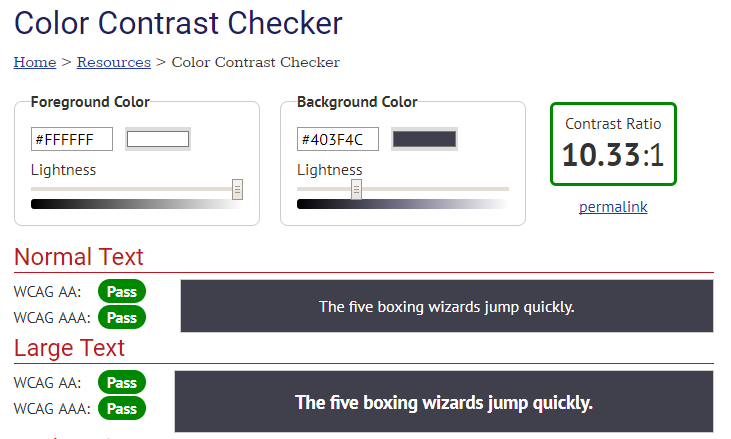
\includegraphics[height=6cm]{images/contrast-checker.png}\\
			\caption{A screenshot taken from \citep{contrast-check} displaying the results from checking the Colour Contrast on \nt. The hex codes for the two main colours of the design is entered into the ``Foreground Color'' and ``Background Color'' boxes, the results are displayed below.}\label{fig:contrast-check}
		\end{figure}
		
		\subsection{Considerations towards Developers} \label{sec:devcons}
		Usability and Accessibility is not an issue that concerns only the users of a system. The developers have to invest significant time and resources into integrating Operating System level features, such as the iOS Magic Touch, into their apps. Unfortunately, many developers underestimate the increase in complexity that accessibility brings. This can lead to projects being exceeding their budget and time limits.
		
		This is why for the development of \nt, React Native was chosen. React Native is a cross platform JavaScript library that has integrated many of the Operating System level accessibility features into itself \citep{reactAccess}. Due to this integration, we can override the default screen readers with more informative labels, or set the iOS Magic Tap to perform specific tasks, both of which will be addressed in greater detail in Section \ref{sec:nortrav}.
		
	% EOF Usability and Accessibility Discussion
	% BOF NorwichTravel overview
	\section{\nt} \label{sec:nortrav}
	As we learned in Section \ref{sec:scenario}, \nt \ was developed through the use of a Scenario. The Scenario is broken down into a list of \textit{User Stories} that is then translated into a list of functionality for the app. There are two main advantages to developing through Scenarios; it is a simple method to generate functionality, but more importantly it places the user at the centre of the app from the very start of the development cycle. See Section \ref{sec:prop-func} for a full list of proposed functionality from the Scenario.
	
	From Section \ref{sec:devcons}, we learned that \nt \ is a React Native app. Allowing for easy Cross-Platform (iOS and Android) support and rapid prototyping when used in conjunction with services such as Expo. In addition to the support that React Native has for accessibility functionality (see Section \ref{sec:devcons}).
	
		\subsection{Proposed Functionality} \label{sec:prop-func}
		\nt \ is an app that provides public transport information for Norwich. The three principle forms of public transport within Norwich are Buses, Trains and Taxis. Below is the list of functionality related to information about the aforementioned public transport:
			\begin{itemize}
				\item Look up Bus Times from a Bus Stop within Norwich.
				\item Look up the next Train Times from Norwich Station.
				\item Look up the time of the next Train from Norwich to a given location.
				\item Find a list of Taxi companies that operate within Norwich. 
			\end{itemize} 
		
		\subsection{Target Audiences} \label{sec:target}
		From the Scenario in Section \ref{sec:scenario} we can tell that \nt \ is aimed principally at the Students of UEA. However, \nt \ can be used by anyone who needs by transport information within Norwich, be it Business Personnel on a trip to Norwich or a tourist passing through whilst exploring the Norfolk Broads. This means that we are looking at a very diverse user base. Individuals of all backgrounds and skill sets could use \nt. Therefore the design of \nt \ must be focused on Usability. 
		
	% EOF NorwichTravel overview
	% BOF Design Discussion
	\section{Designing for Usability and Accessibility} \label{sec:design}
	As we discussed in Section \ref{sec:industry}, there is a set of guidelines provide assistance to developers when integrating accessibility features. In addition to the W3 Accessibility Guidelines, the BBC have released a comprehensive guide to accessibility in apps \citep{bbcguide}.
	
	In this section we will discuss some examples from these two guidelines and how they relate to \nt, with a further investigation into the compromises made to conform to the industry standard guidelines.
	
		\subsection{Conforming to Guidelines} \label{sec:conform}
		\textbf{Guideline 1: Colour Contrast} - mentioned in both of the guidelines we are concerning ourselves with. A ratio of \textbf{4.5:1} is supplied that reflect the contrast that should exist between the Foreground Text and Background Colour. To conform to this guideline we aimed to have the colour scheme of \nt \ double this metric, having a minimum contrast \textbf{9:1}. This makes \nt \ highly accessible to those who are visually impaired.
		
		\textbf{Guideline 2: Touch Target Size} - inspired by the W3 Accessibility Guidelines and expanded by the BBC Mobile Accessibility Guidelines. The metric to aim for is a touch target area (i.e. a button) must be between \textbf{7-10mm height and width}. In addition to the expected design elements such as the buttons must not overlap.
		
		\textbf{Guideline 3: Text Size} - defined within the mobile section of the W3 Accessibility Guidelines, it dictates that the default text should be able to be doubled in size without loosing content. \nt \ text was defined with this in manner and text will wrap to prevent any loss of content.
		
		\subsection{Compromises Made} \label{sec:comp}
		\nt \ was designed with Usability and Accessibility in mind from the conception of the app. Due to this the design compromises that to be made were minimal. Those that had to be made are the expansion of the Train \textit{search component} and the choice of React Native. 
		
		The \textit{search component} within \nt \ is shared between both the Bus and Train containers. The Bus container only takes an origin for the search function. The Train screen however can take either an origin or an origin and destination combined. This subtle change in the search component functionality caused the developers measurable increase in hours spent on the project. The compromise here is that whilst it might be easier to implement two search components, in terms of maintainability it was better to have one - despite the increase in development time.
		
		The choice of React Native was a compromise between the ease of development and the ability to access the operating system native accessibility features. This allowed \nt \ to respond to the system settings for text size and allowed the developers to set specific labels for the screen readers to vocalise. 
		
	% EOF Design Discussion
	% BOF Evaluation and Testing
	\section{Evaluating \nt} \label{sec:eval}
	\nt \ used Continuous Integration (CI) and Continuous Deployment (CD) tools such as Expo and CodeShip. This allows for the latest version of the app to be tested without the developers having to manually redeploy after each commit to the GitHub repository. 
	
	The general methodology for testing was to use the industry standard tools when possible (see Section \ref{sec:industry-tools}), the ``glasses'' test as often an possible (see Section \ref{sec:glasses}) and Think-Aloud evaluations during milestones within the project. Milestones for \nt \ are defined by major features being ``completed''. For example; the bus search functionality working would be a milestone, and would be the testing of the bus search would include a Think-Aloud Evaluation. Prototyping was used at the start of the development cycle (see Section \ref{sec:proto}), to avoid costly and time consuming mistakes further into the project.
	
		\subsection{Prototyping} \label{sec:proto}
		Lo-fi prototyping involves sketching the design of a system on paper, whilst producing labels to overlay the design to mock how the final system will operate. As stated in Section \ref{sec:eval}, the lo-fi was used at the begining of the development cycle to quickly refine the initial concepts. These prototypes can be seen in Appendix \ref{app:lo-fi}.
		
		Med-fi prototyping was used throughout the development process through the use of emulators such as Genymotion and Simulator. This allowed the developers to ``live preview'' the changes they were making as if they were running on a mobile device. The emulator tools could mimic a large range of mobile devices so that all screen sizes could be tested. The final version of the app was published using expo, examples of this can be seen in Appendix \ref{app:final}.
			
		\subsection{``Glasses'' Test} \label{sec:glasses}
		Both of the developers working of \nt \ posses diminishing eyesight. At the suggestion of the Project Supervisor, one of the principle testing methods that was employed throughout \nt's development cycle was the ``Glasses'' Test. A developer to load the app on a phone, through Expo, and remove their glasses. The phone would be positioned in such a way that it became hard to see. The developer would have to then complete a set of tasks with and without the screen reader active. Any issues that were encountered could be noted immediately by the developer. 
		
		This test proved extremely effective, due to its similarity to the Think-Aloud Evaluation. The crucial difference is that the developer does not have to convey their thoughts to an evaluator. Instead they can note down the issues they encounter in a manner that makes sense to them and then immediately act upon them. 
		
		\subsection{Industry Tools} \label{sec:industry-tools}
		As we learned from Figure \ref{fig:contrast-check}, WebAIM's contrast checker was used to certify that \nt \ was accessible to those with visual impairments. 
		
	\section{Issues within \nt} \label{sec:major}
	One of the largest issues within \nt \ was the state of affairs within React Native's conditional rendering. The search component is an abuse of turnery statements and generally poor coding practice, which was unavoidable. This leaves the search component in a state of disarray where it is neither a component nor a container in the traditional manner.
	
	Further issues for \nt \ was the lack of support for developing an accessible and usable mobile app. Websites have a multitude of testing platforms that inform developers exactly what parts of their system is not complying with W3 Accessibility Guidelines. The only tool that we could borrow from the Website Industry was the contrast checker, as discussed \ref{sec:industry-tools}.
	
	Finally we have uncovered two larger-scale issues with accessibility and usability within the mobile app industry. Developers are those who interact with software the most. Currently accessibility and usability is focused on the users, which is not incorrect. However, if the focus would to shift slightly to develop tools that increase the maintainability of accessible and usable features. It would incentivise the developers to spend more time on perfecting these features.
	
	However, should accessibility and usability features be called features? The industry as a whole need to recognise that accessibility and usability is something that should be a part of every single app and website. Not a selling point.
	% EOF Evaluation and Testing
	% BOF Conclusion
	\section{Conclusions} \label{sec:conc}
	In conclusion, throughout this paper we have explored the process of developing a mobile app with the express purpose of being Usable and Accessible. Examining the guidelines and documentation that supports the process of integrating accessibility. Investigated the testing methodologies and techniques that are suited towards accessibility and usability functionality. We have looked into the advantages of React Native and using the Operating System level functions. Finally we have discussed the issues that were noted during the development of \nt, including two wider issues across the industry.
	
		\subsection{Was \nt \ fit for purpose?} \label{sec:fit}
		The functionality proposed in Section \ref{sec:prop-func} were met, as evidenced by the screenshots in Appendix \ref{app:final}.
		
		\subsection{Was \nt \ accessible to the target user groups?} \label{sec:accessibletotarget}
		\nt \ met all the relevant accessibility and usability criteria that could be sourced from the W3 and BBC guidelines (see Section \ref{sec:industry}). The testing that simulated visual and motor impairments showed positive results. The colour scheme used does not conflict with any colour-blindnesses. With that in mind, it is fair to state that, for the target user groups \nt \ is both accessible and usable. 
		
	% EOF Conclusion
	
	\bibliographystyle{abbrvnat}
	\bibliography{report}
	\clearpage
	\appendix
	\section{Prototypes} \label{app:proto}
		\subsection{Lo-Fi} \label{app:lo-fi}
		\begin{figure}[h]
			\centering
			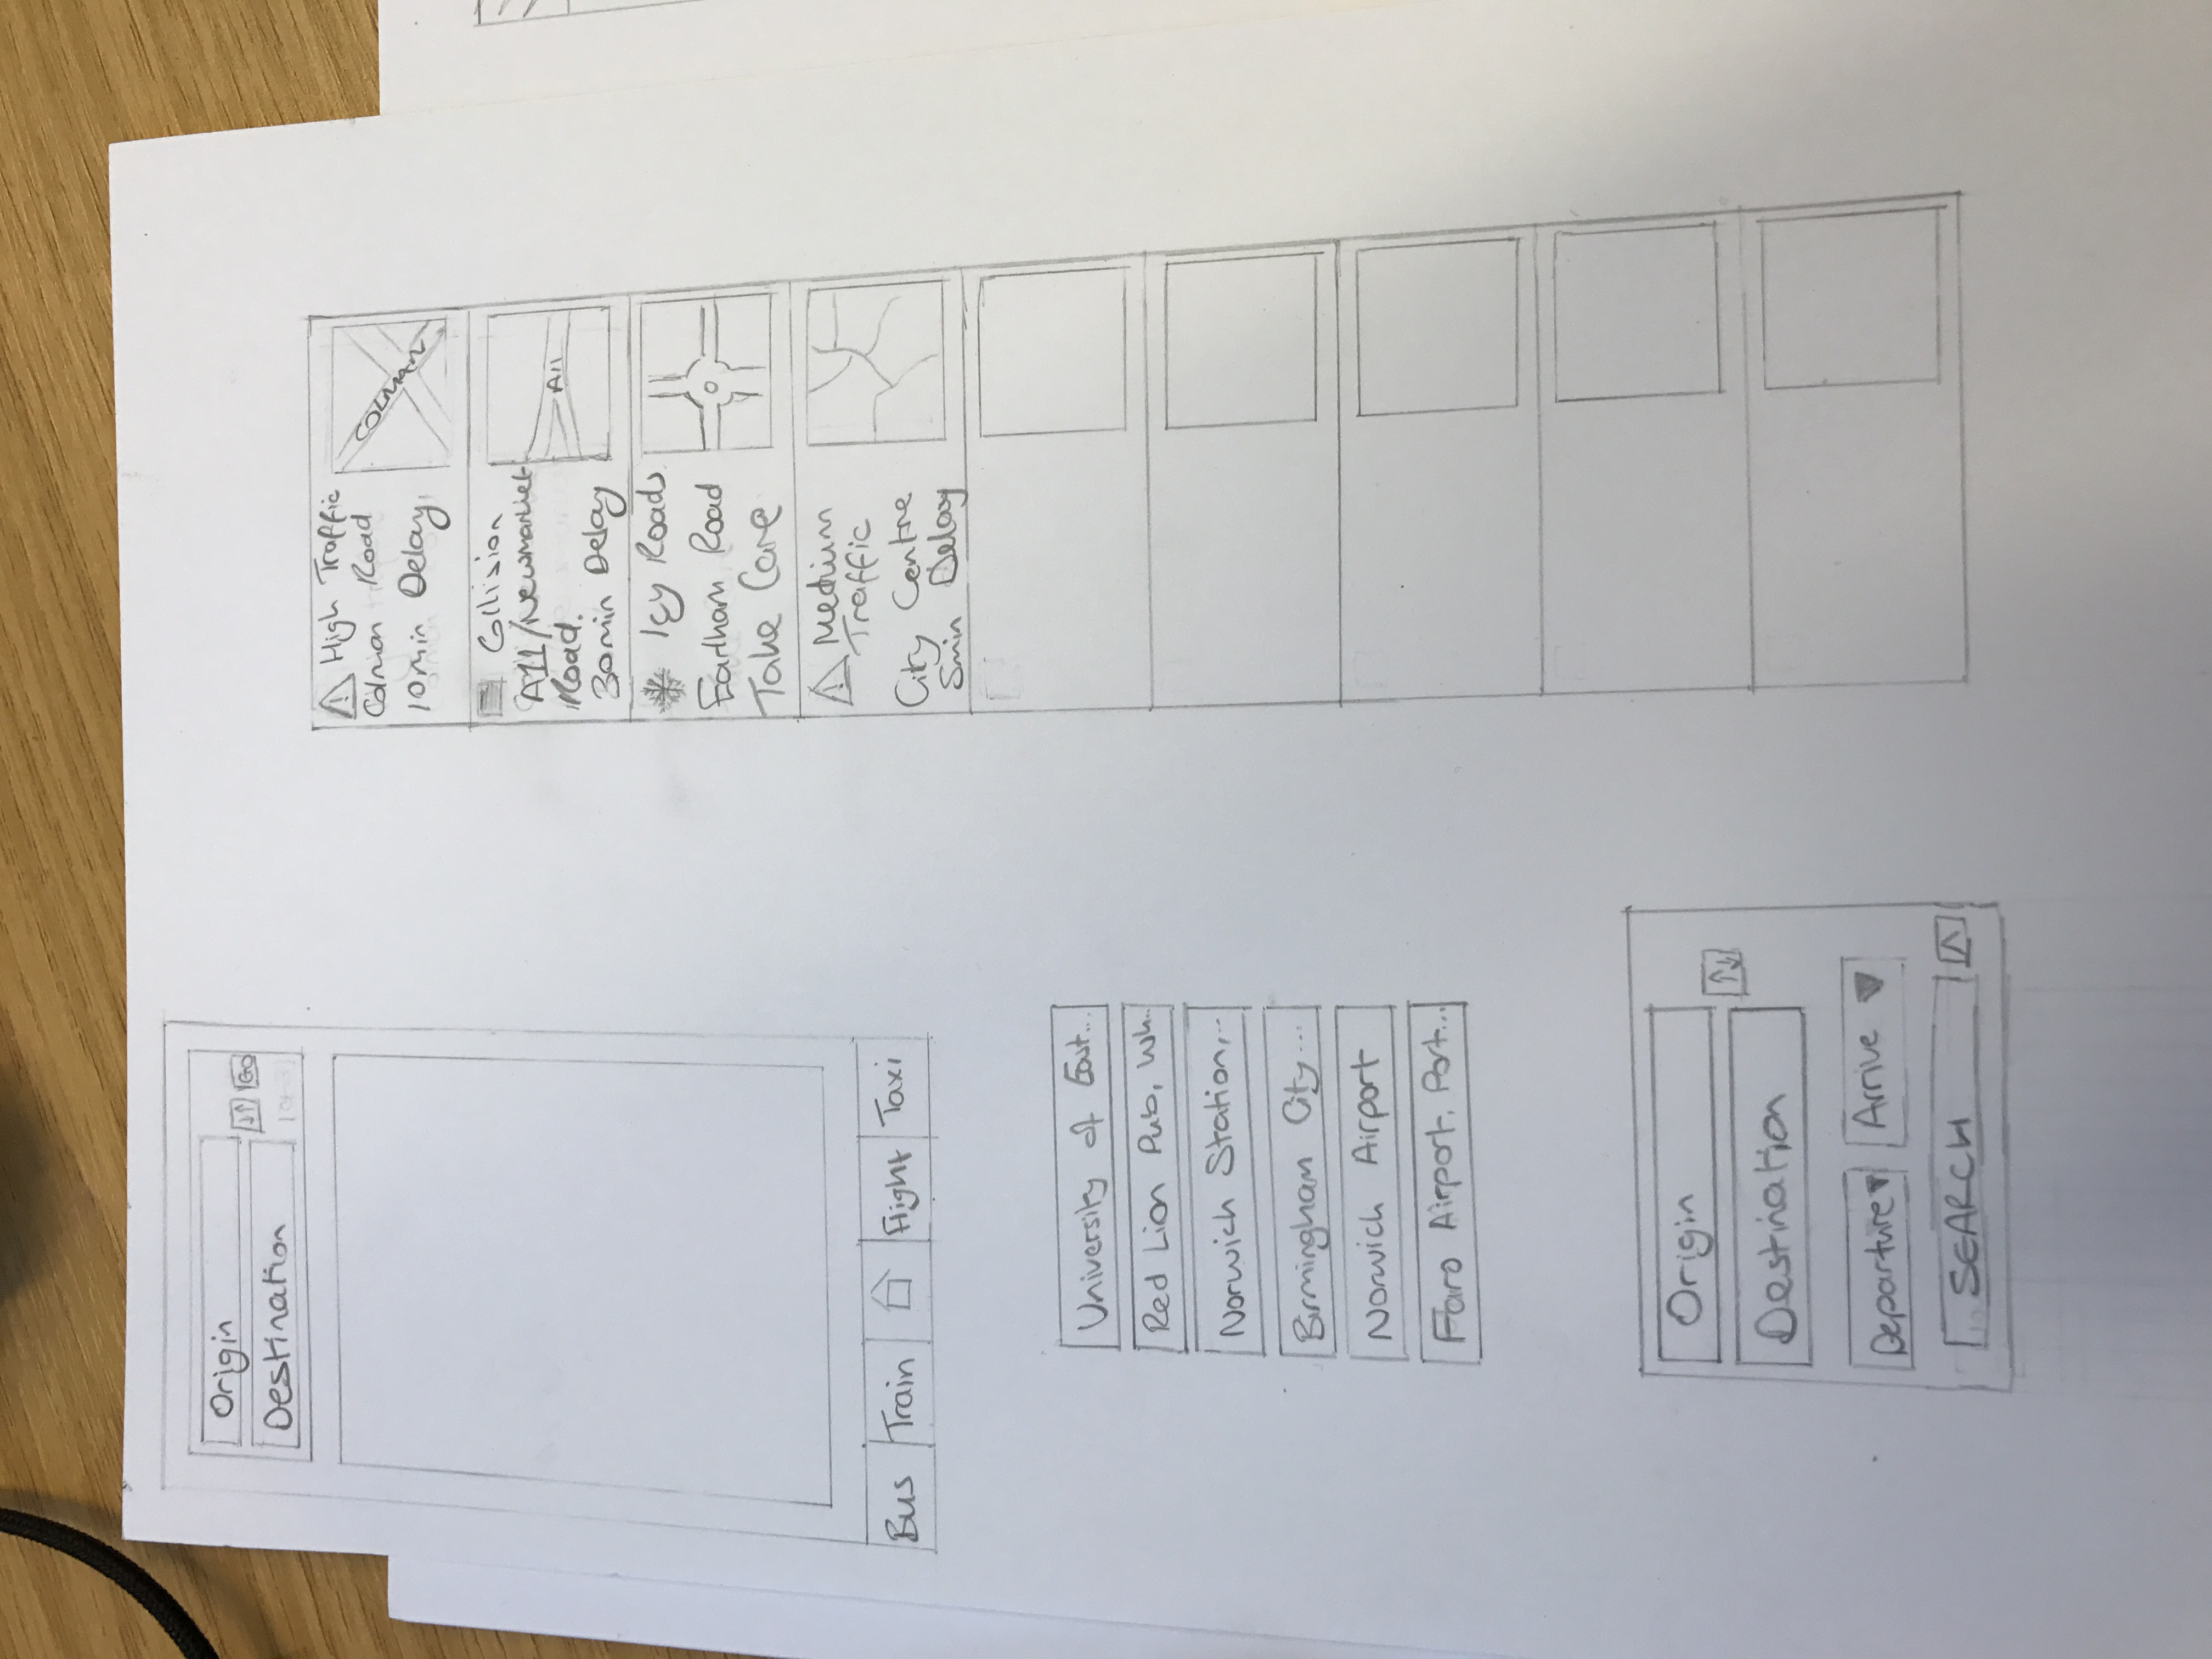
\includegraphics[height=10cm, angle=270]{images/lo-fi-1.jpg}\\
			\caption{Photograph of the development of the lo-fi prototypes of \nt used in early testing.}\label{fig:lo-fi-1}
		\end{figure}
		\begin{figure}[h!]
			\centering
			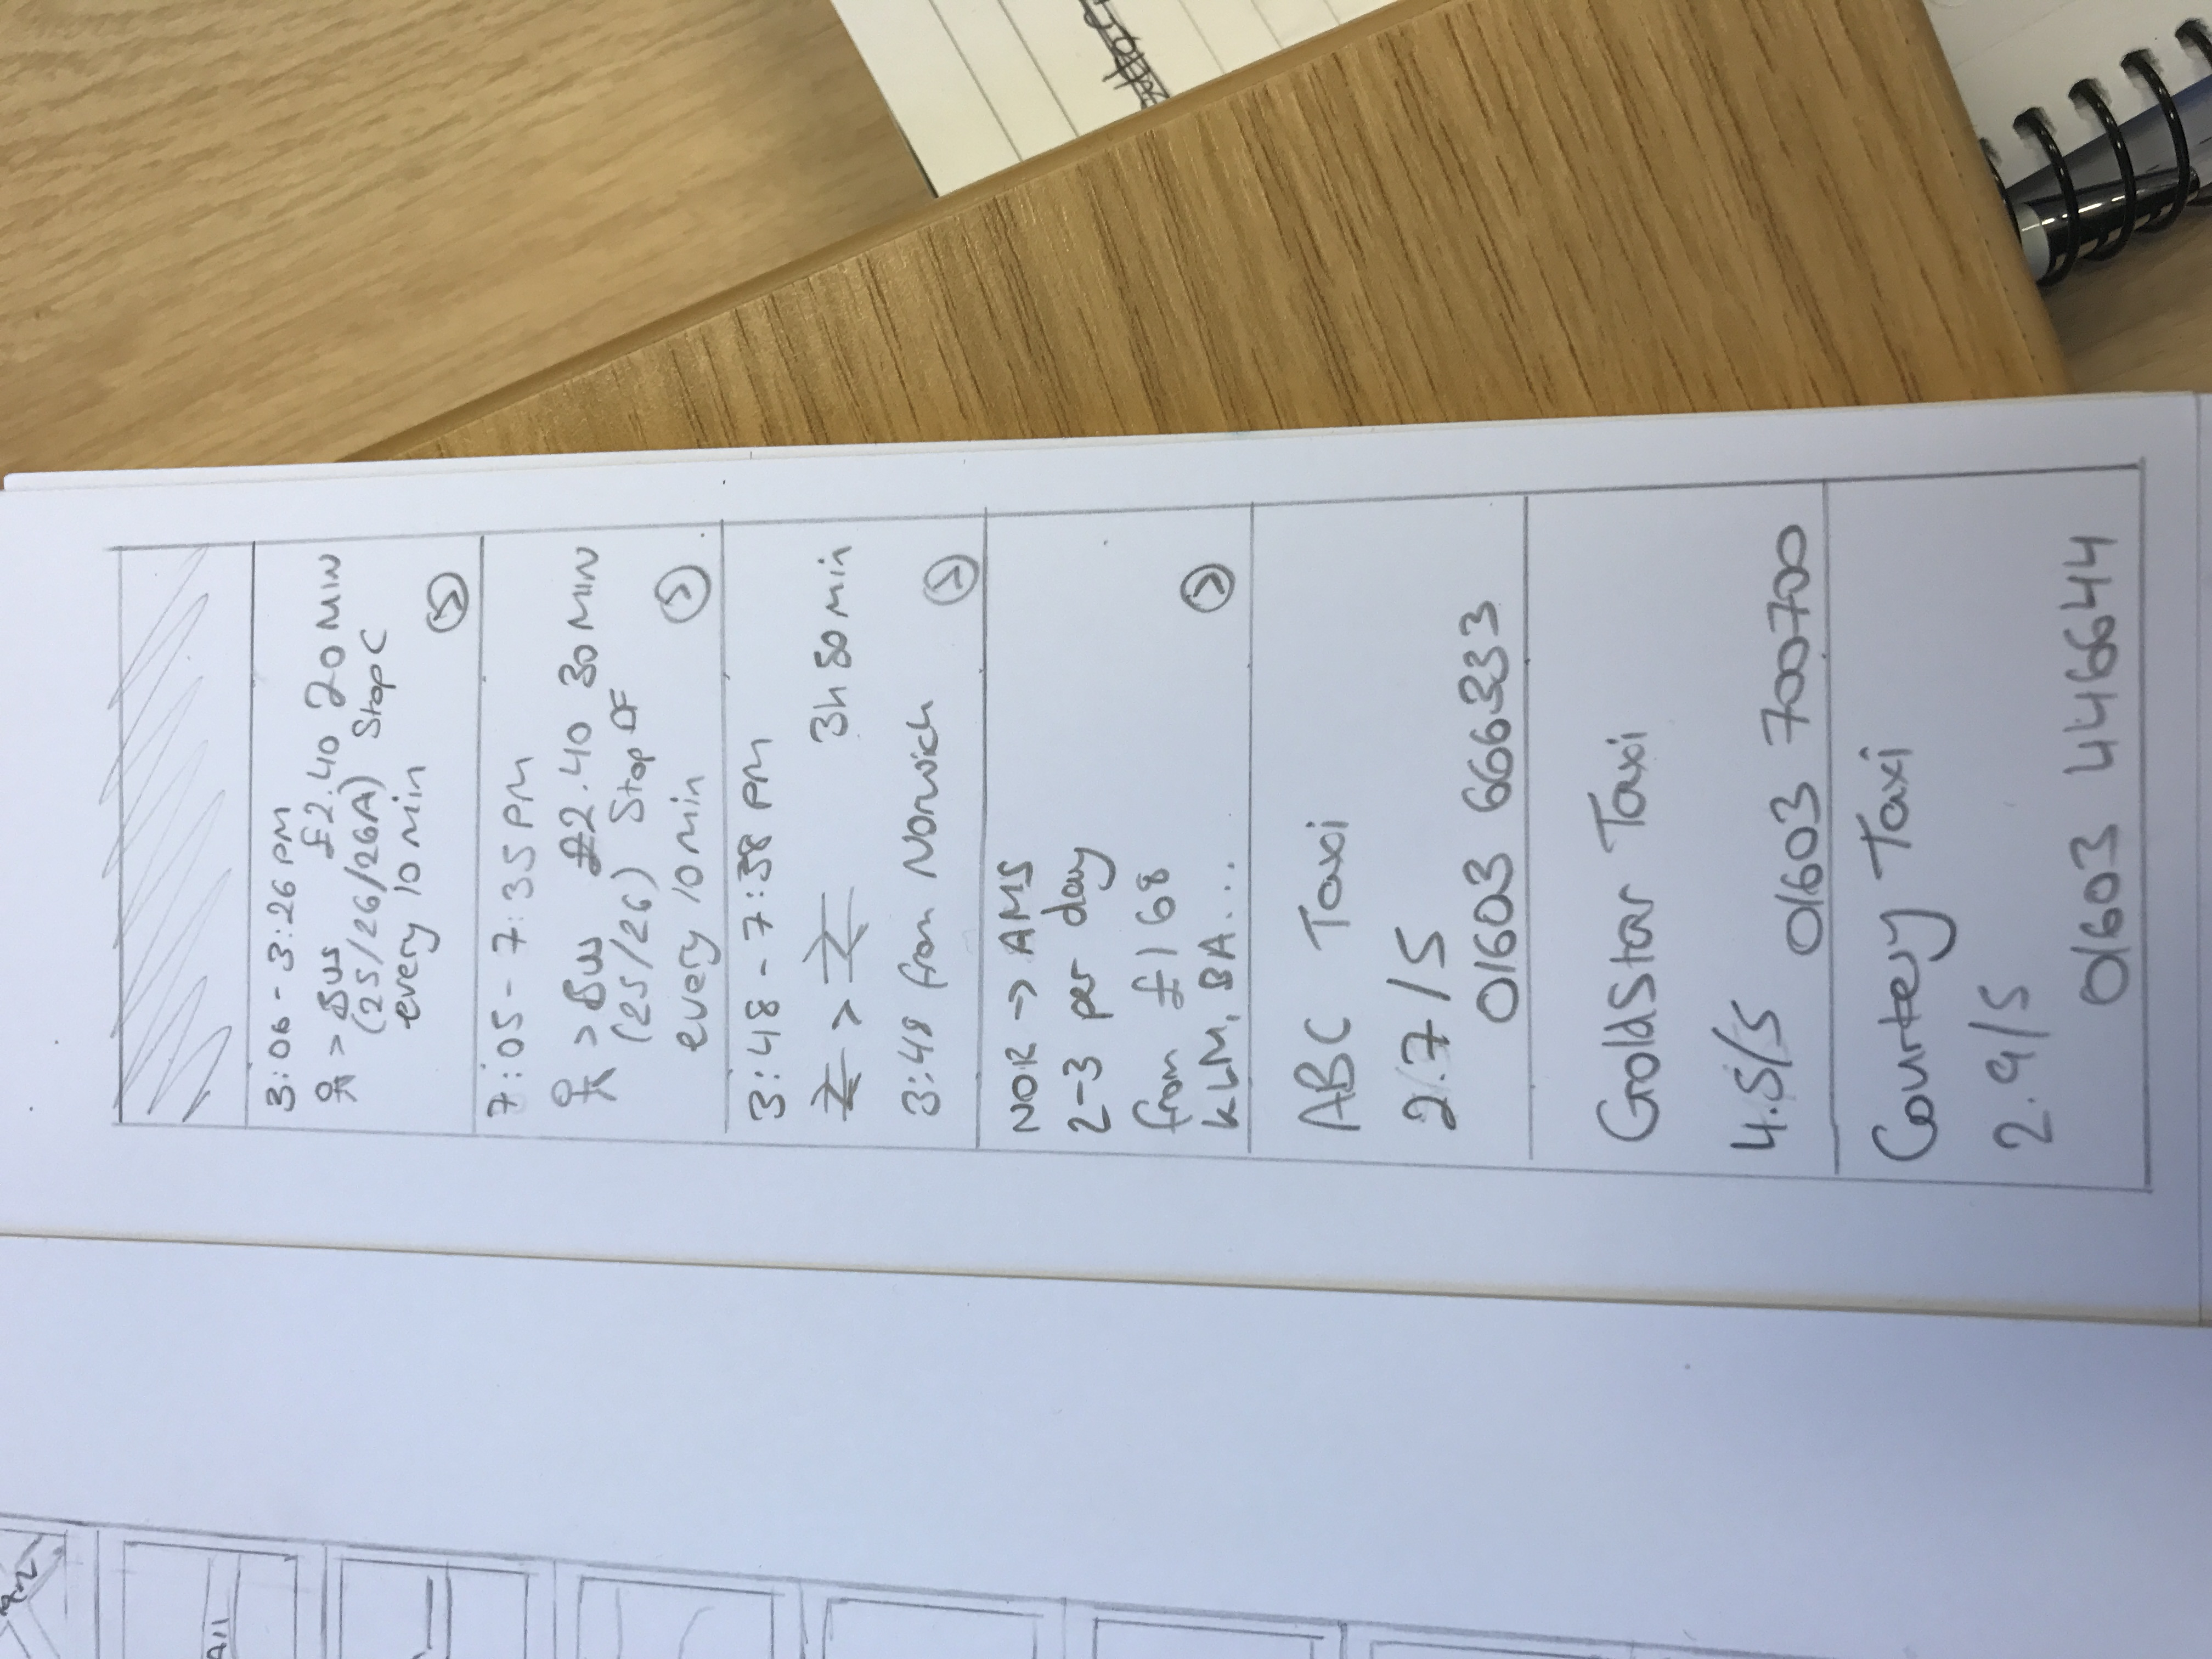
\includegraphics[height=10cm, angle=270]{images/lo-fi-2.jpg}\\
			\caption{Photograph of the development of the lo-fi prototypes of \nt used in aerly testing.}\label{fig:lo-fi-2}
		\end{figure}
		\clearpage
		\subsection{Final System} \label{app:final}
		\begin{figure}[h]
			\centering
			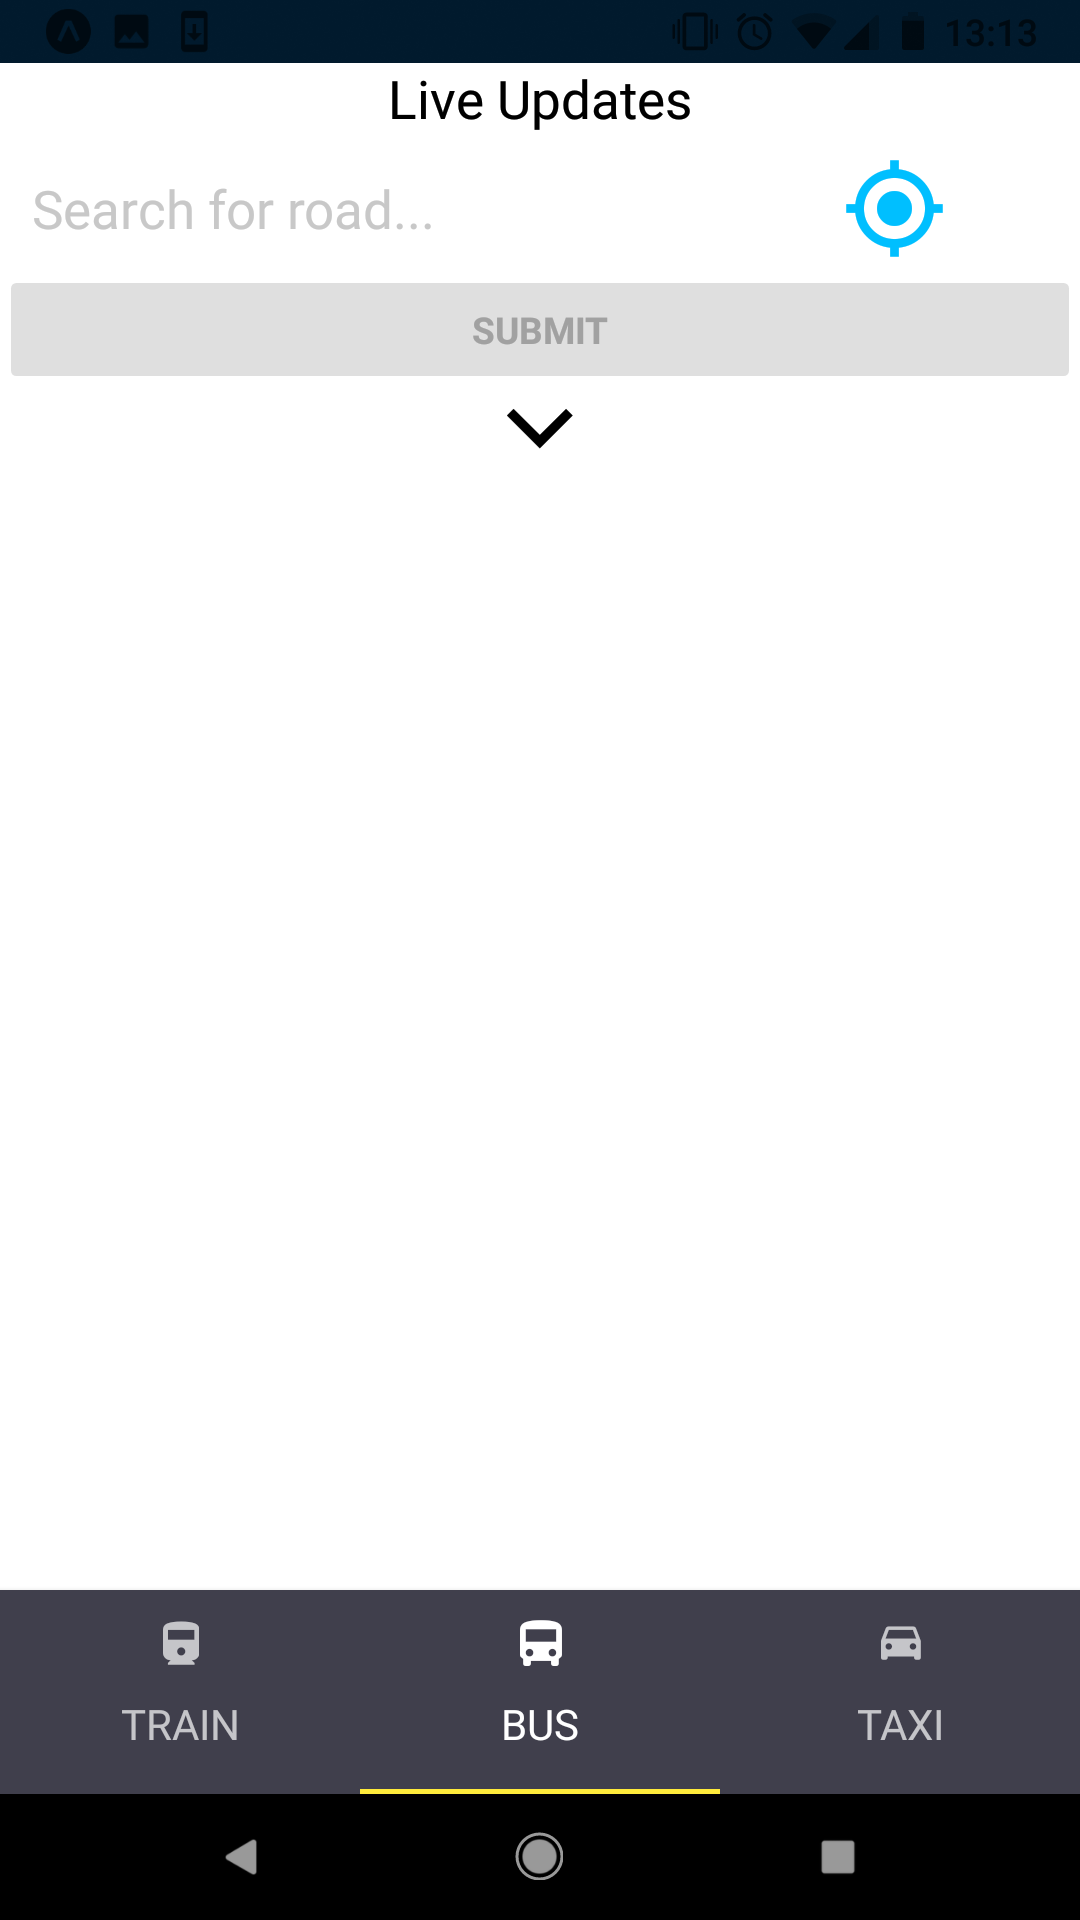
\includegraphics[height=10cm]{images/android-landing.png}\\
			\caption{A screenshot taken from the android version of \nt \ showing the landing page that a User will first see when they open the app.}\label{fig:android-landing}
		\end{figure}
		\begin{figure}[h]
			\centering
			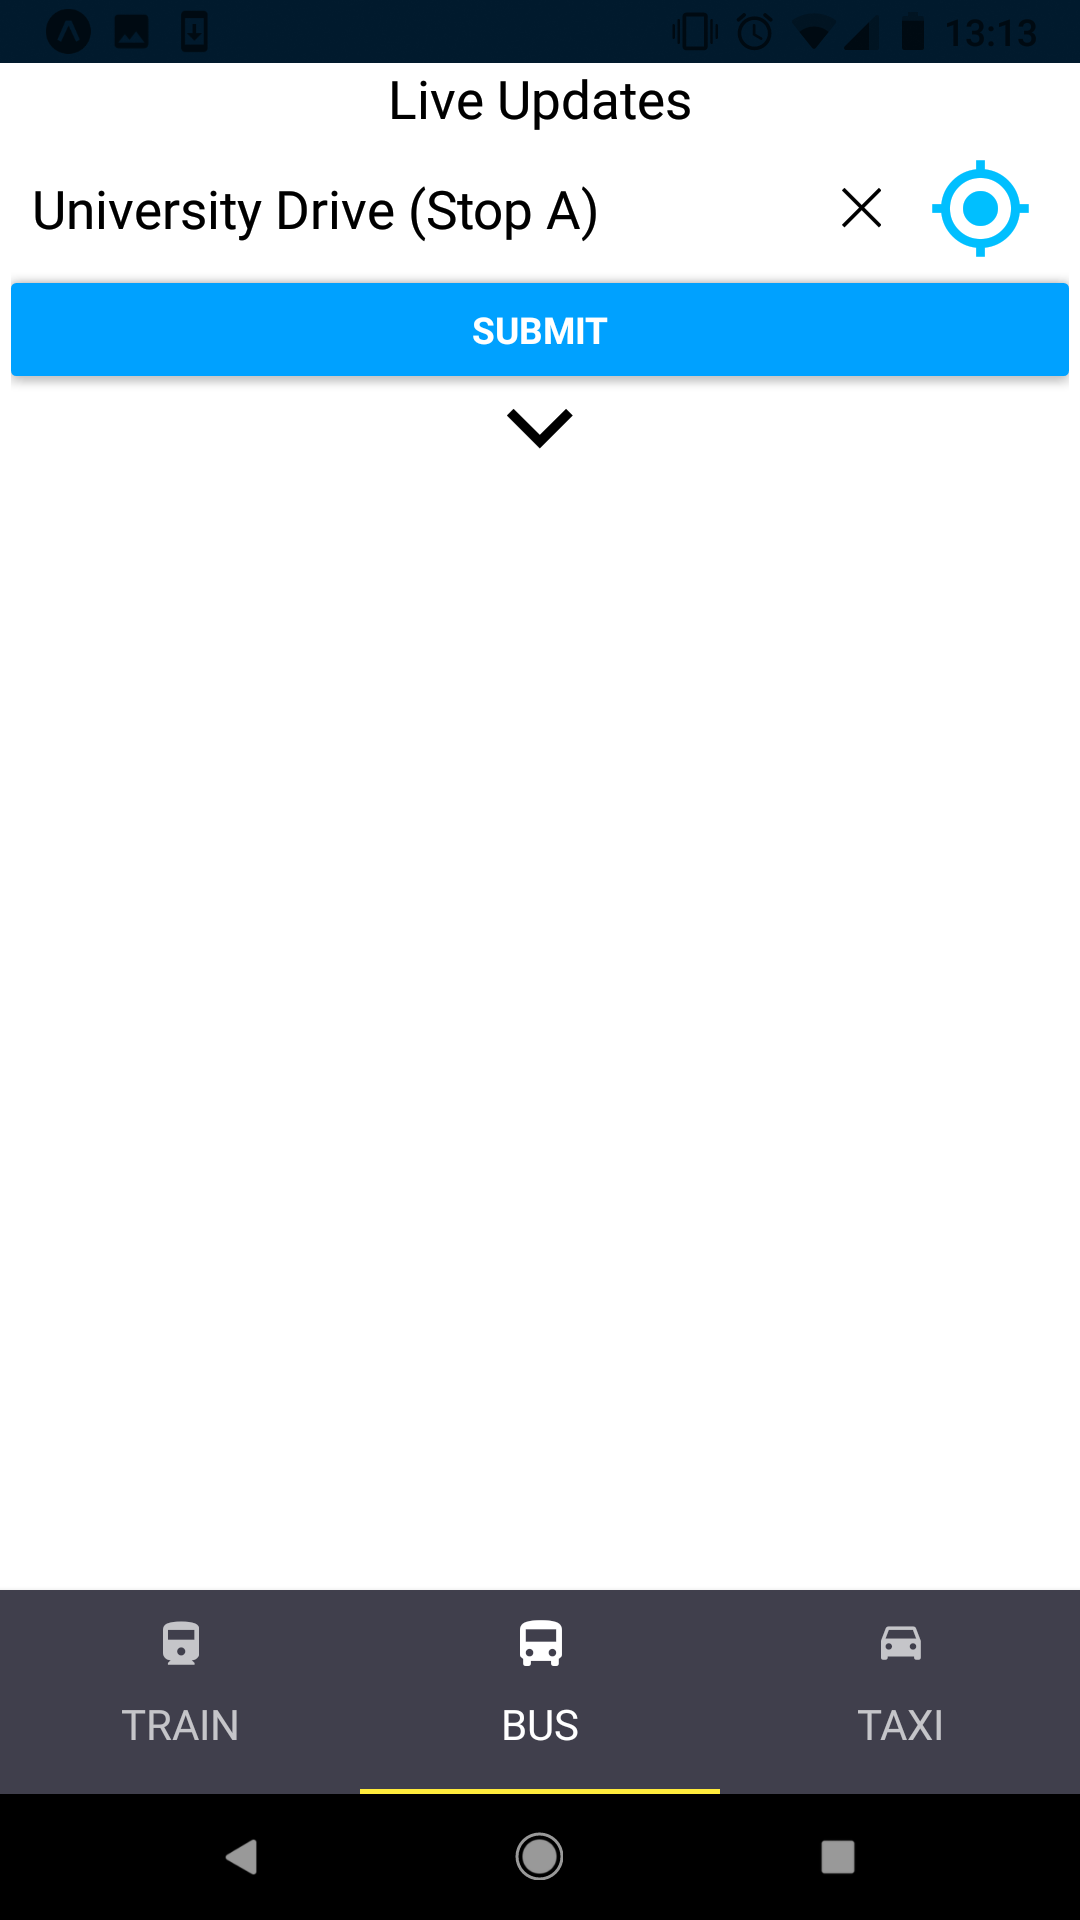
\includegraphics[height=10cm]{images/android-bus-1.png}\\
			\caption{A screenshot taken from the android version of \nt \ showing the Bus Screen with the text field filled.}\label{fig:android-bus-1}
		\end{figure}
		\begin{figure}[h]
			\centering
			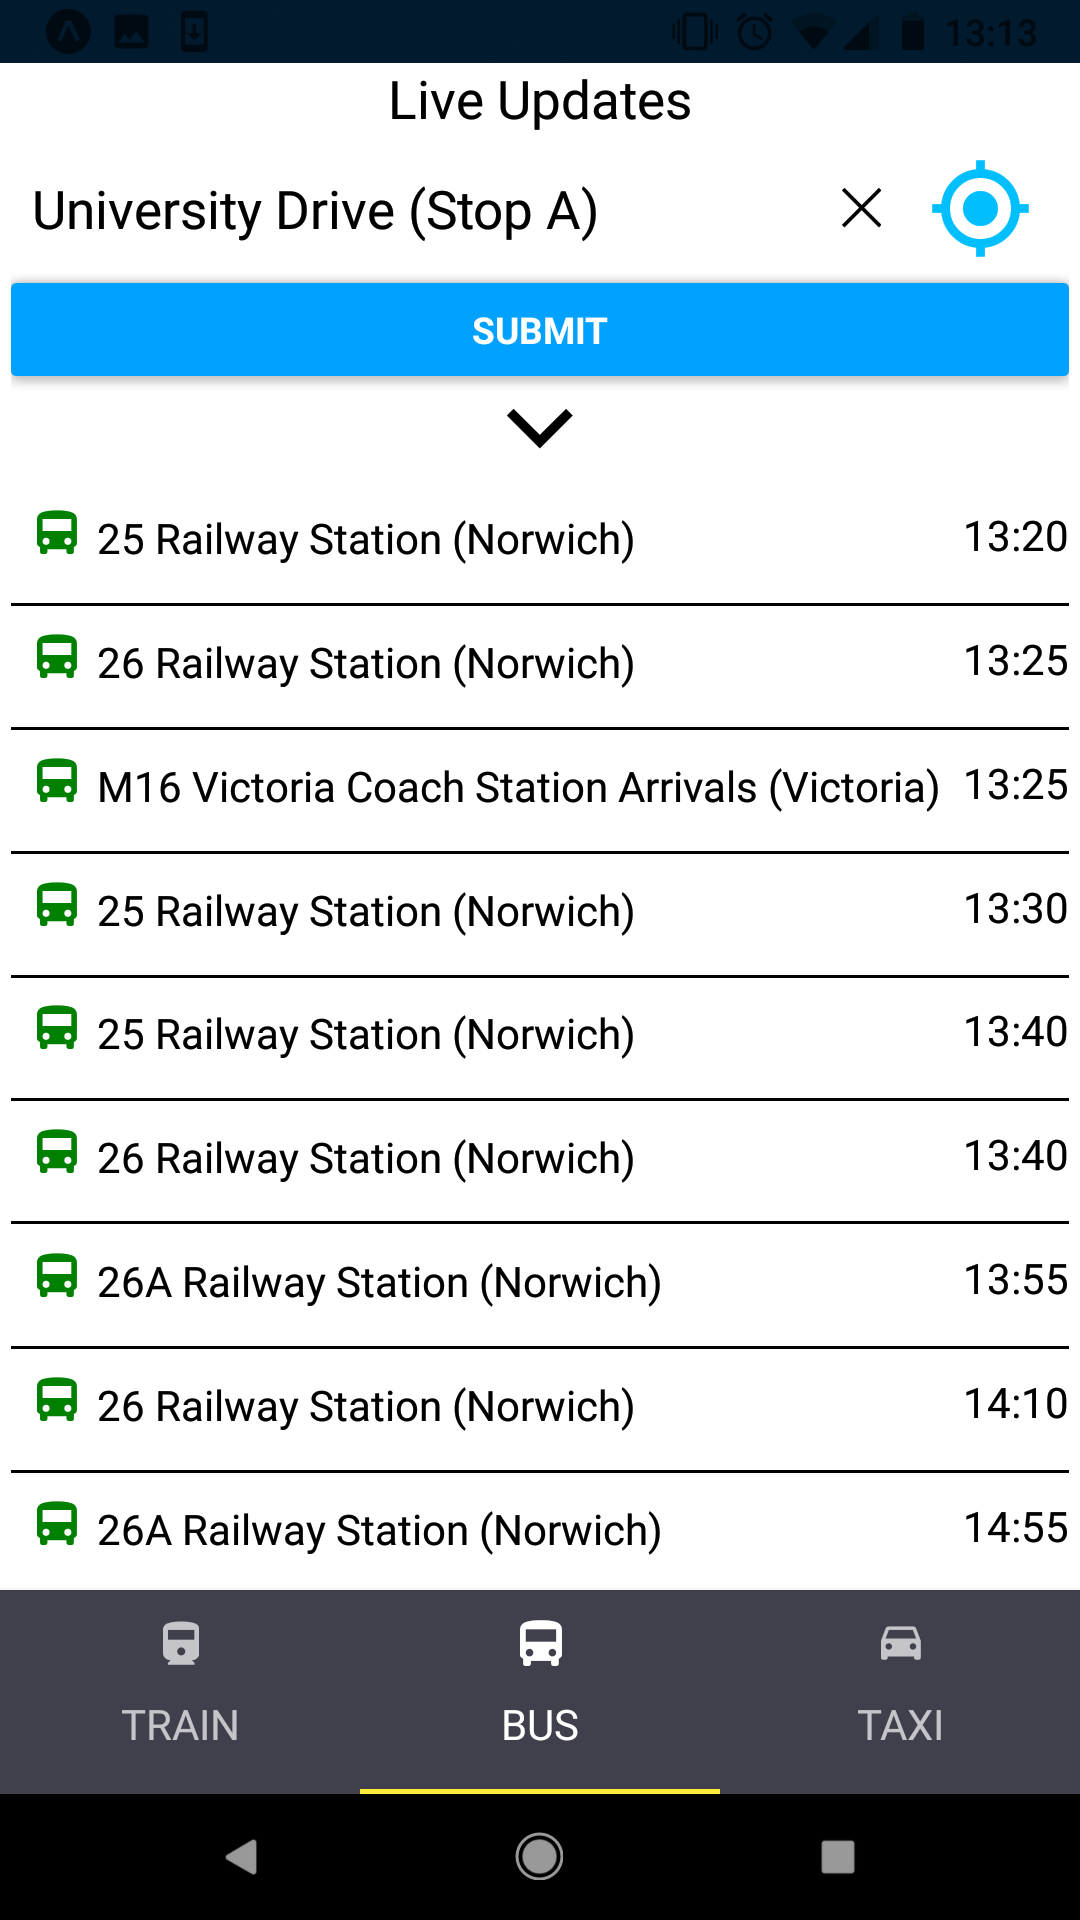
\includegraphics[height=10cm]{images/android-bus-2.png}\\
			\caption{A screenshot taken from the android version of \nt \ showing the Bus Screen with the results generated.}\label{fig:android-bus-2}
		\end{figure}
		\begin{figure}[h]
			\centering
			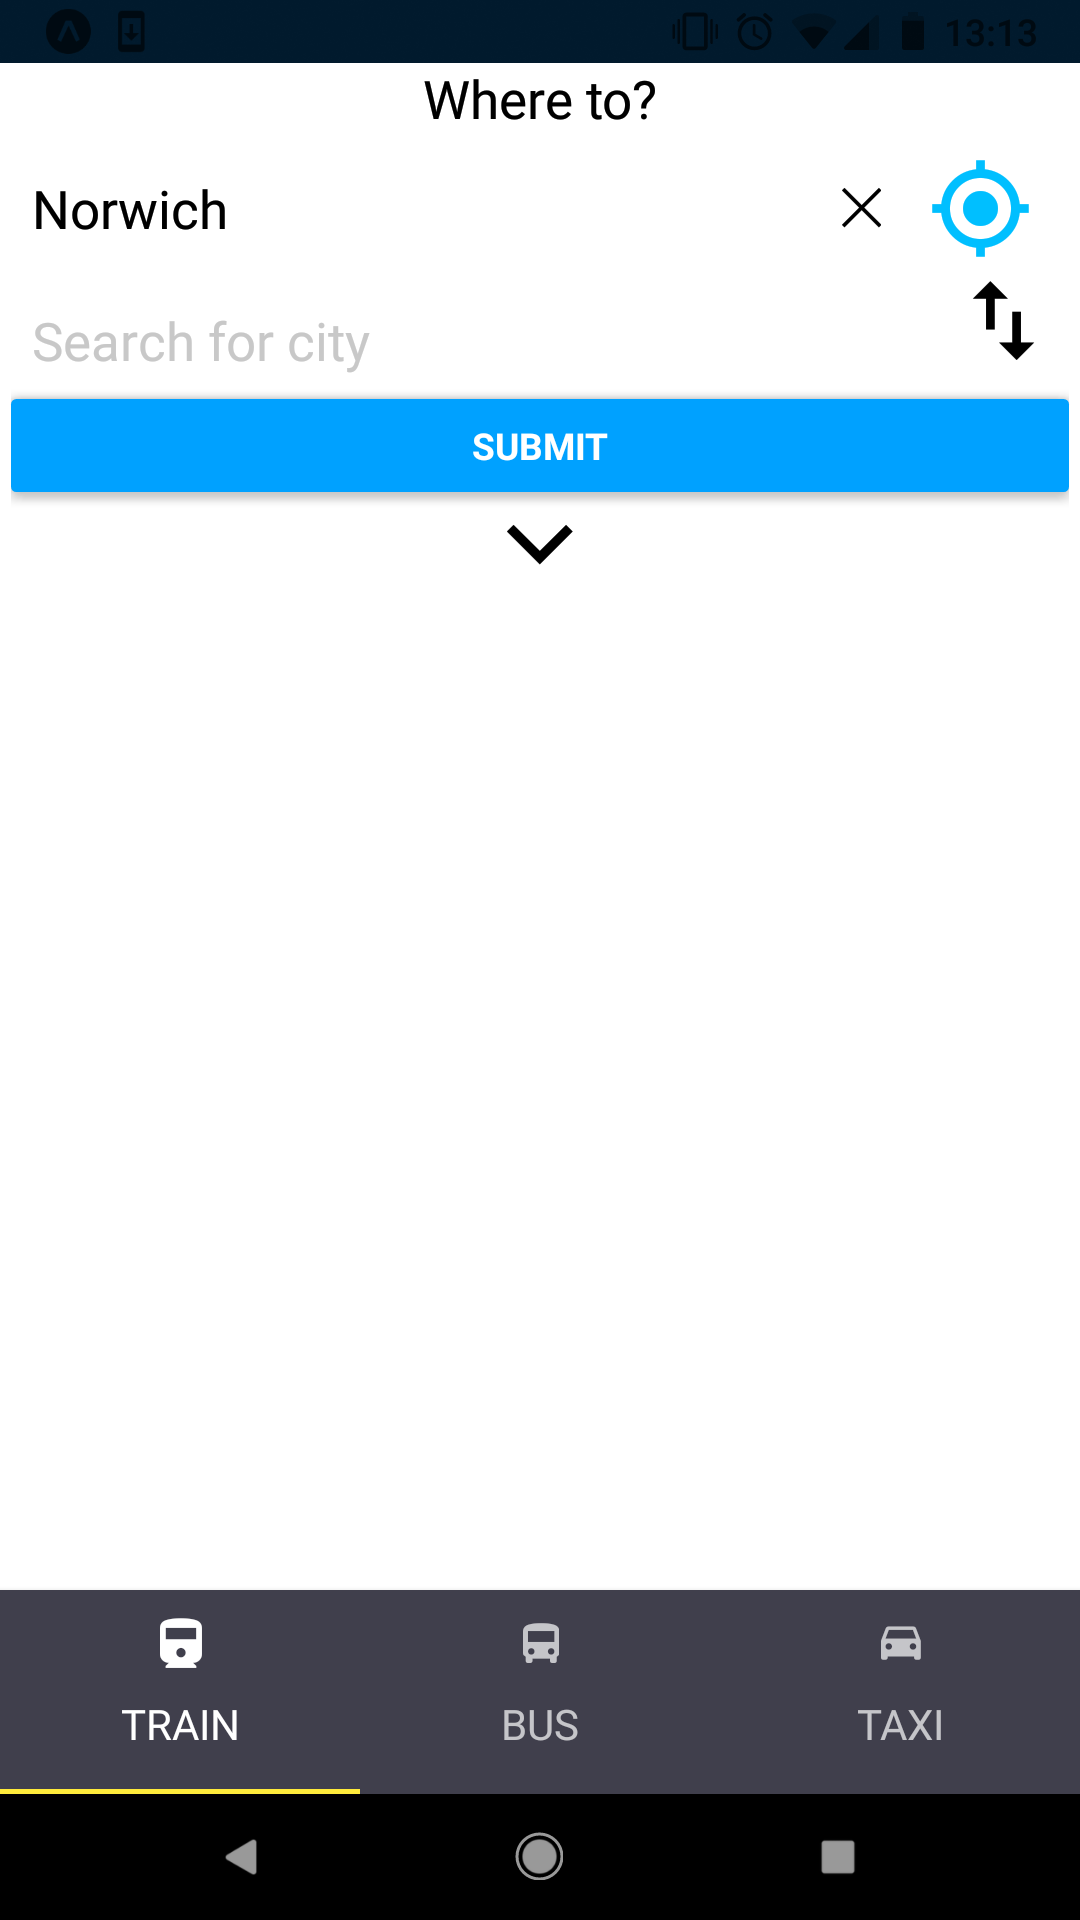
\includegraphics[height=10cm]{images/android-train-1.png}\\
			\caption{A screenshot taken from the android version of \nt \ showing the Train Screen without anything entered. Norwich is the point of origin by default.}\label{fig:android-train-1}
		\end{figure}
		\begin{figure}[h]
			\centering
			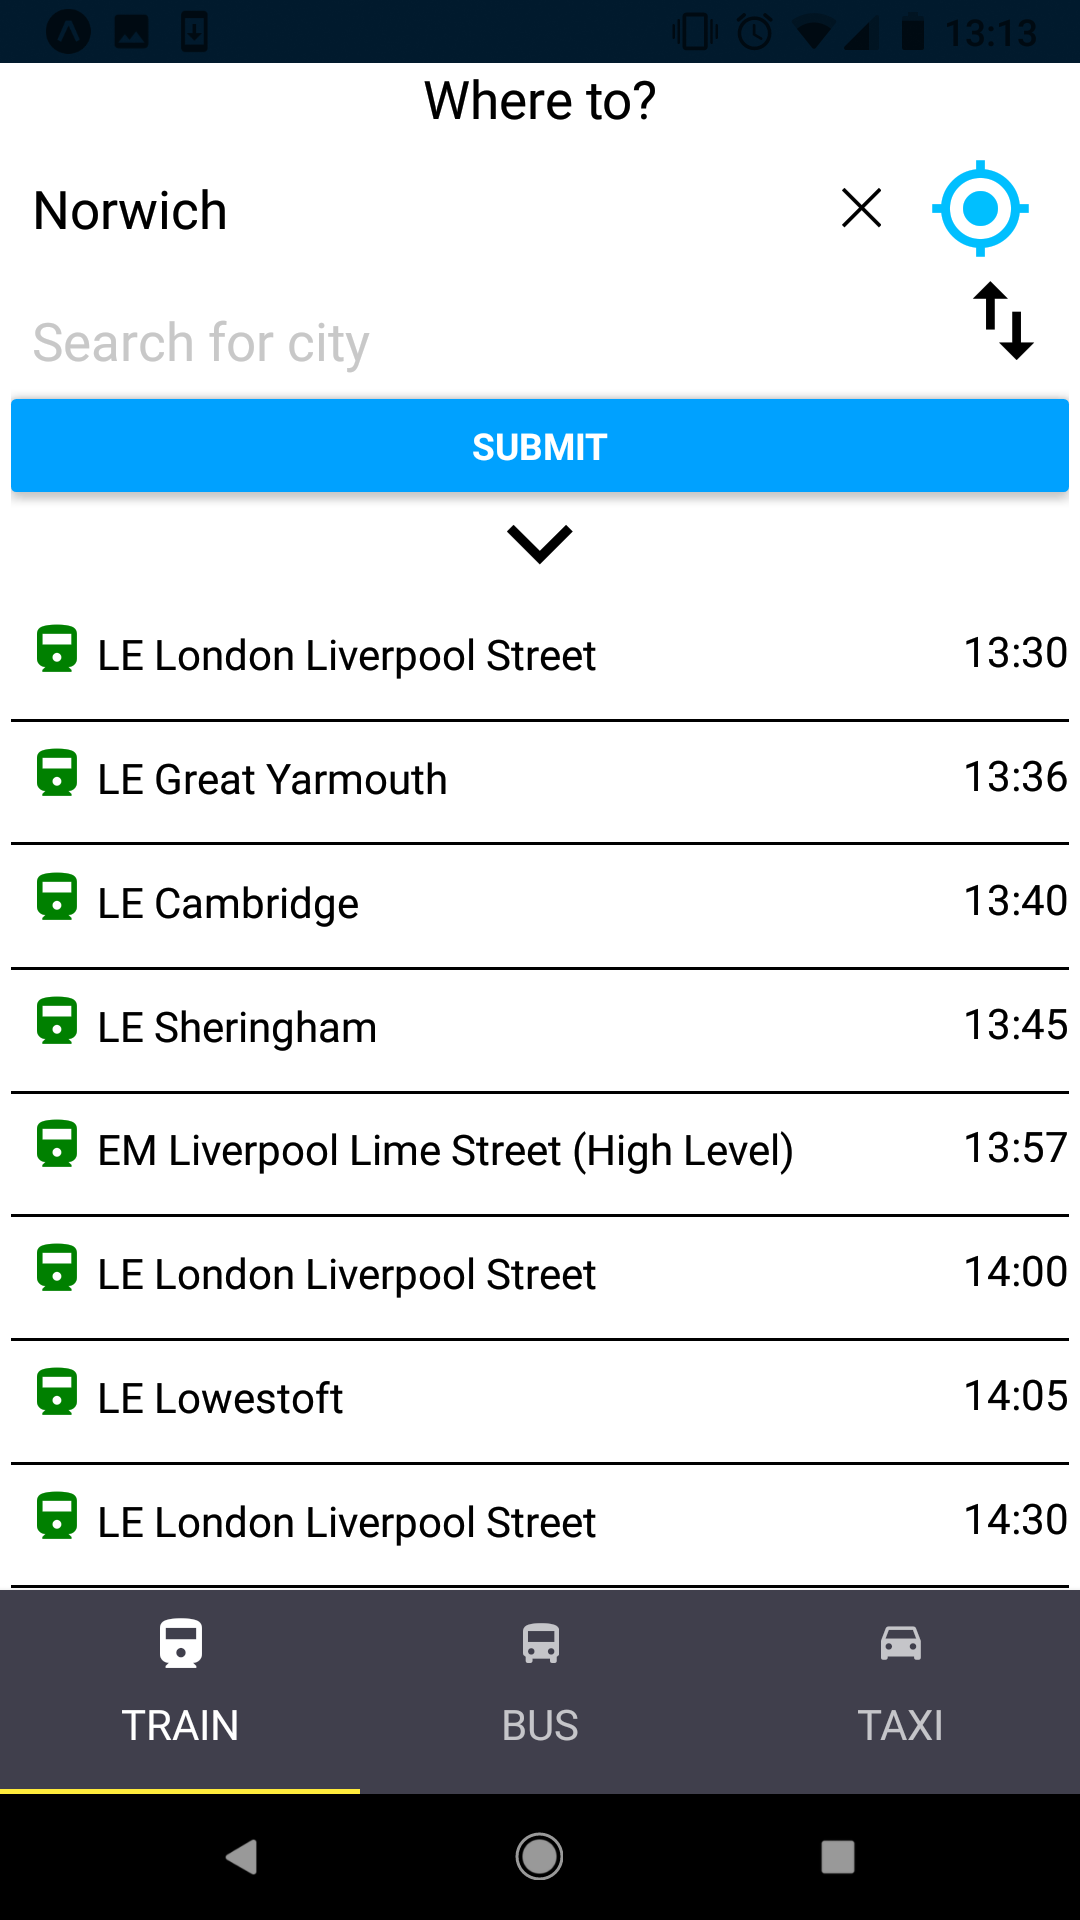
\includegraphics[height=10cm]{images/android-train-2.png}\\
			\caption{A screenshot taken from the android version of \nt \ showing the Train Screen displaying the next rains leaving the station.}\label{fig:android-train-2}
		\end{figure}
		\begin{figure}
			\centering
			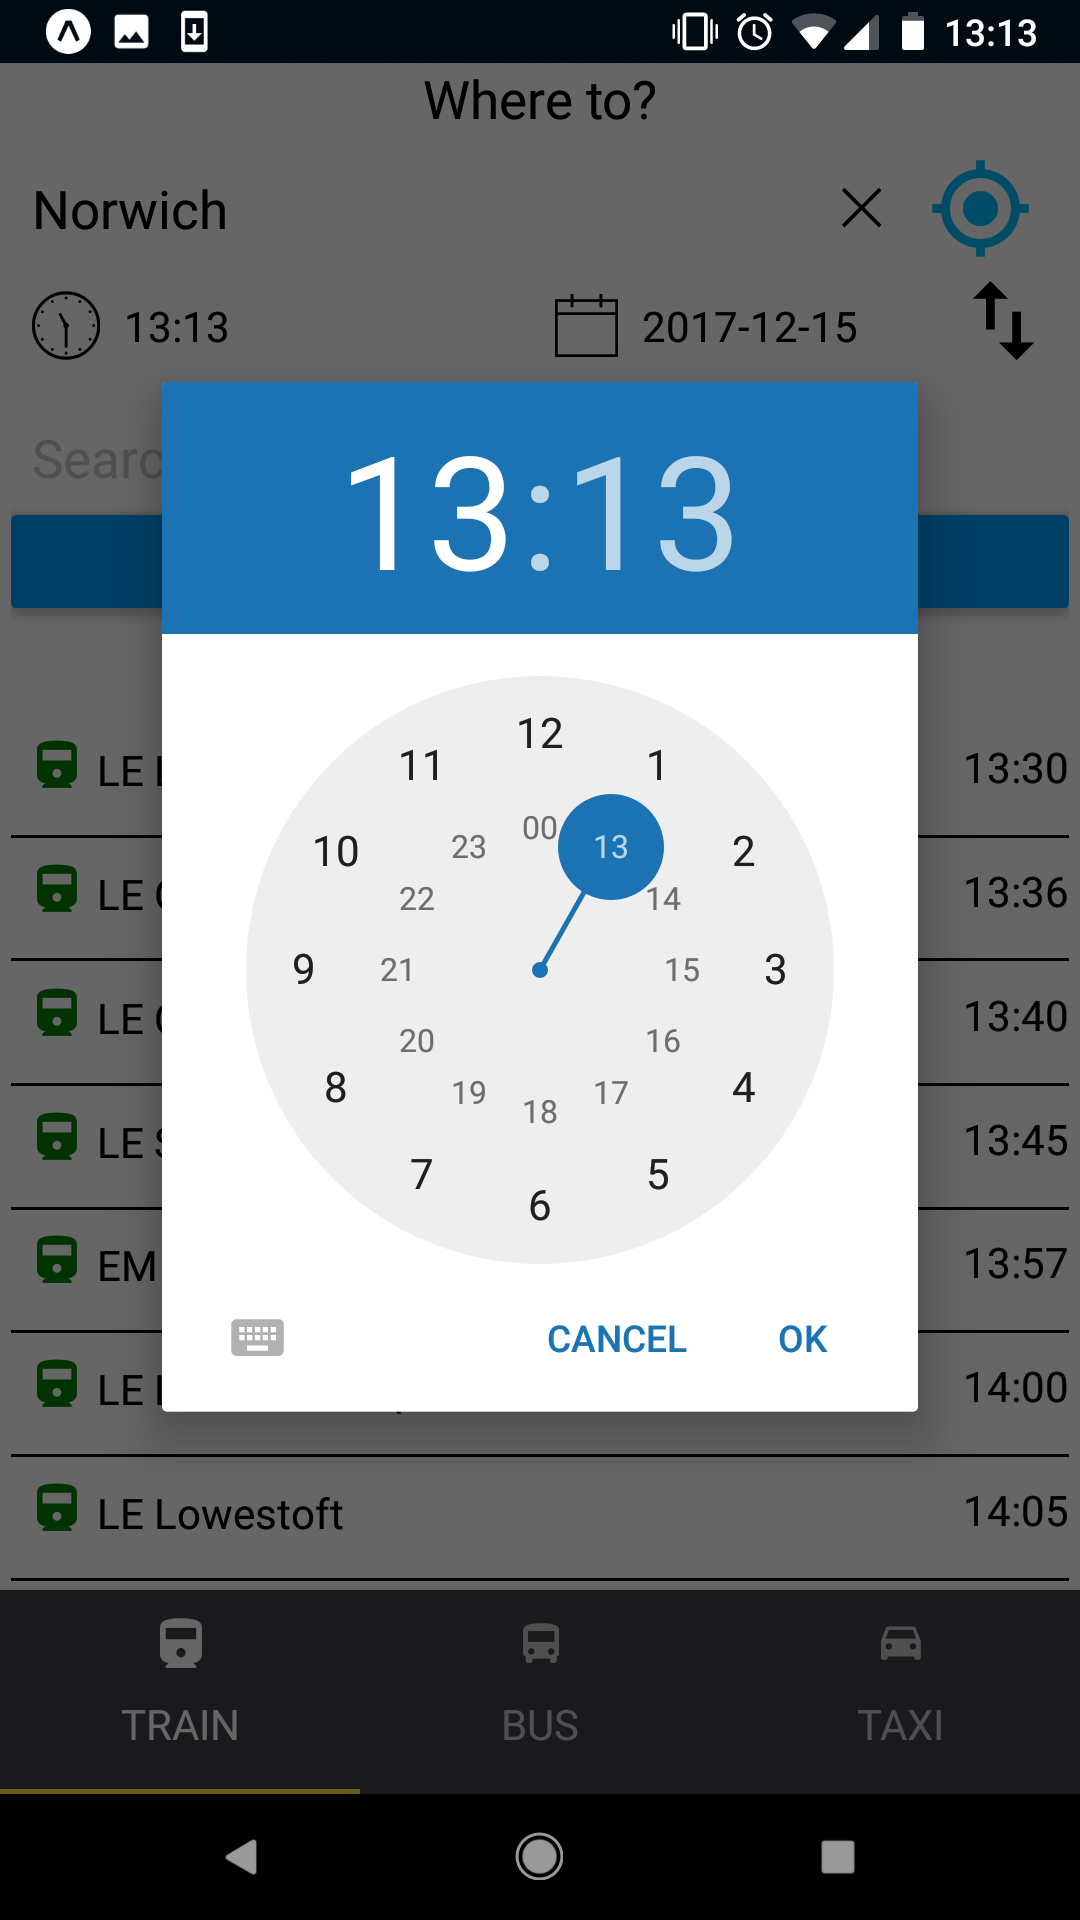
\includegraphics[height=10cm]{images/android-time.png}\\
			\caption{A screenshot taken from the android version of \nt \ showing the Android native time selector.}\label{fig:android-time}
		\end{figure}
		\begin{figure}
			\centering
			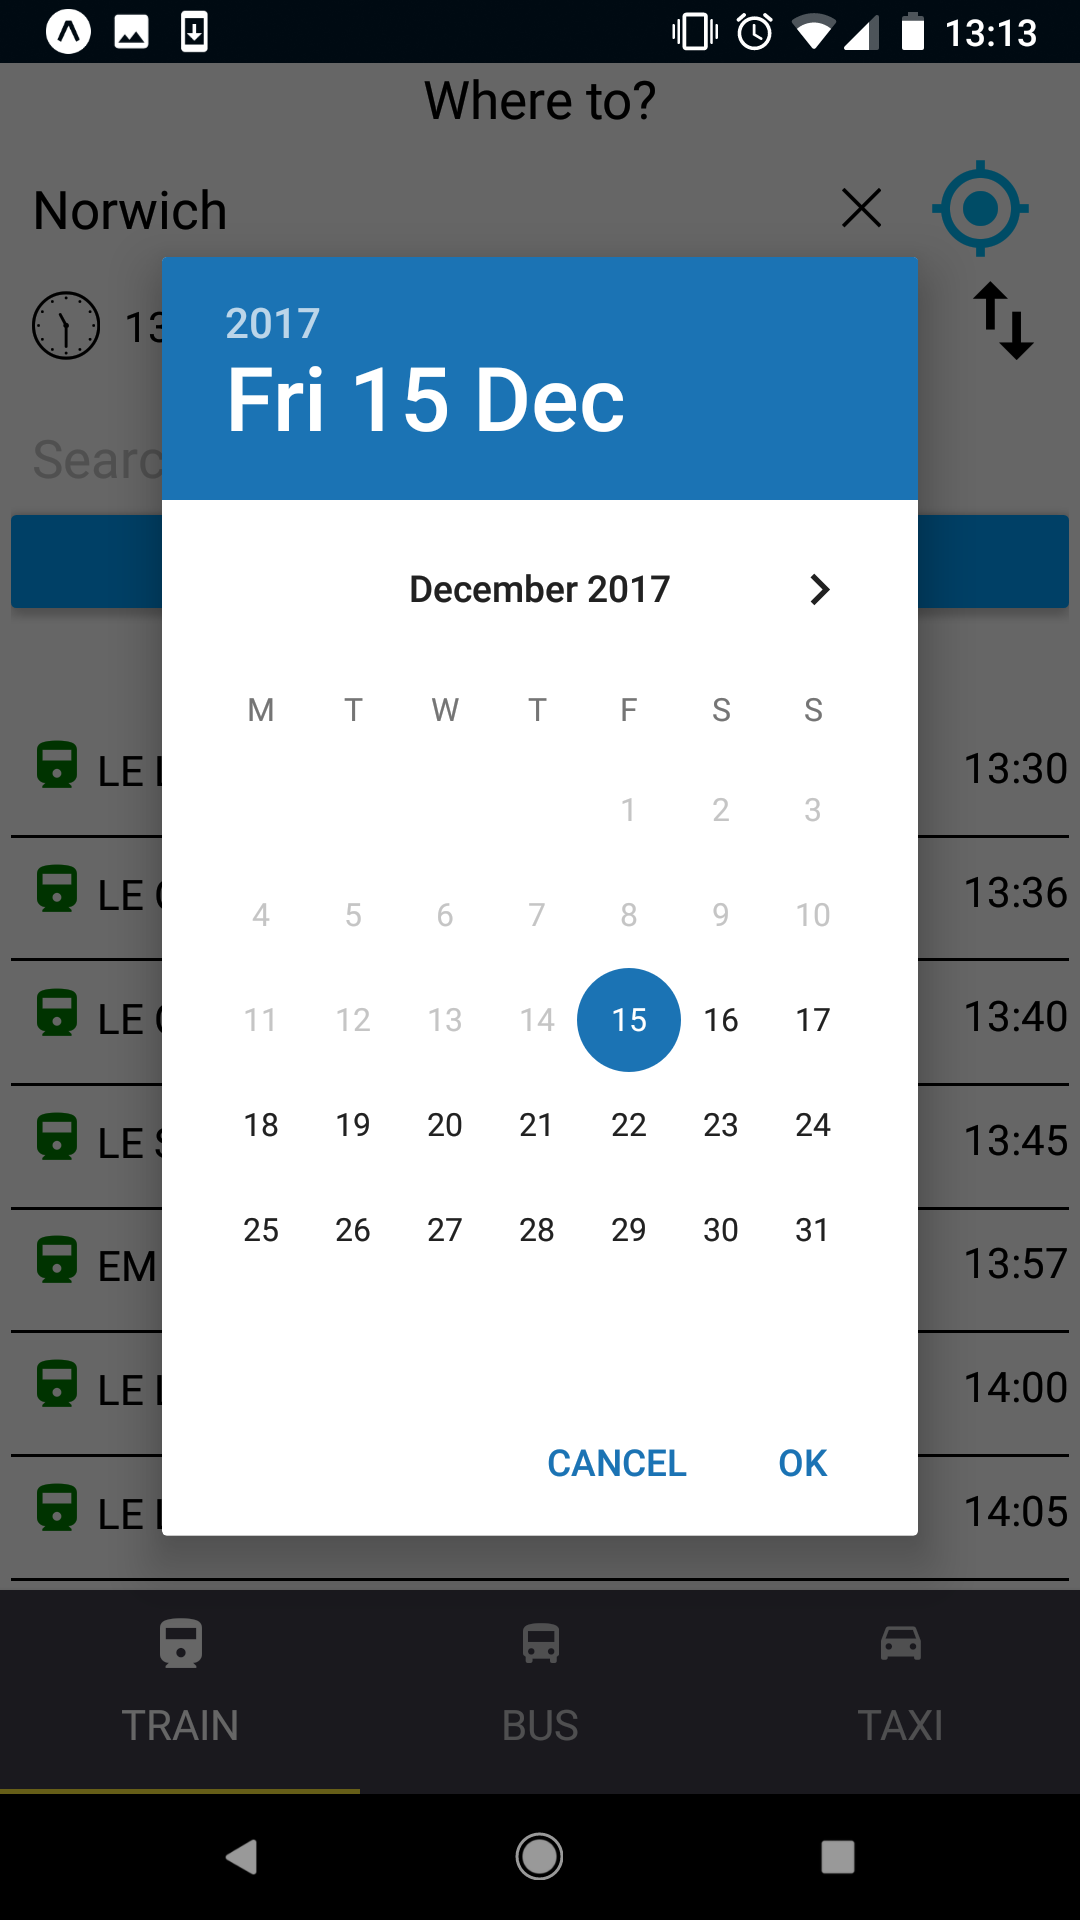
\includegraphics[height=10cm]{images/android-date.png}\\
			\caption{A screenshot taken from the android version of \nt \ showing the Android native date selector.}\label{fig:android-date}
		\end{figure}
		\begin{figure}[h]
			\centering
			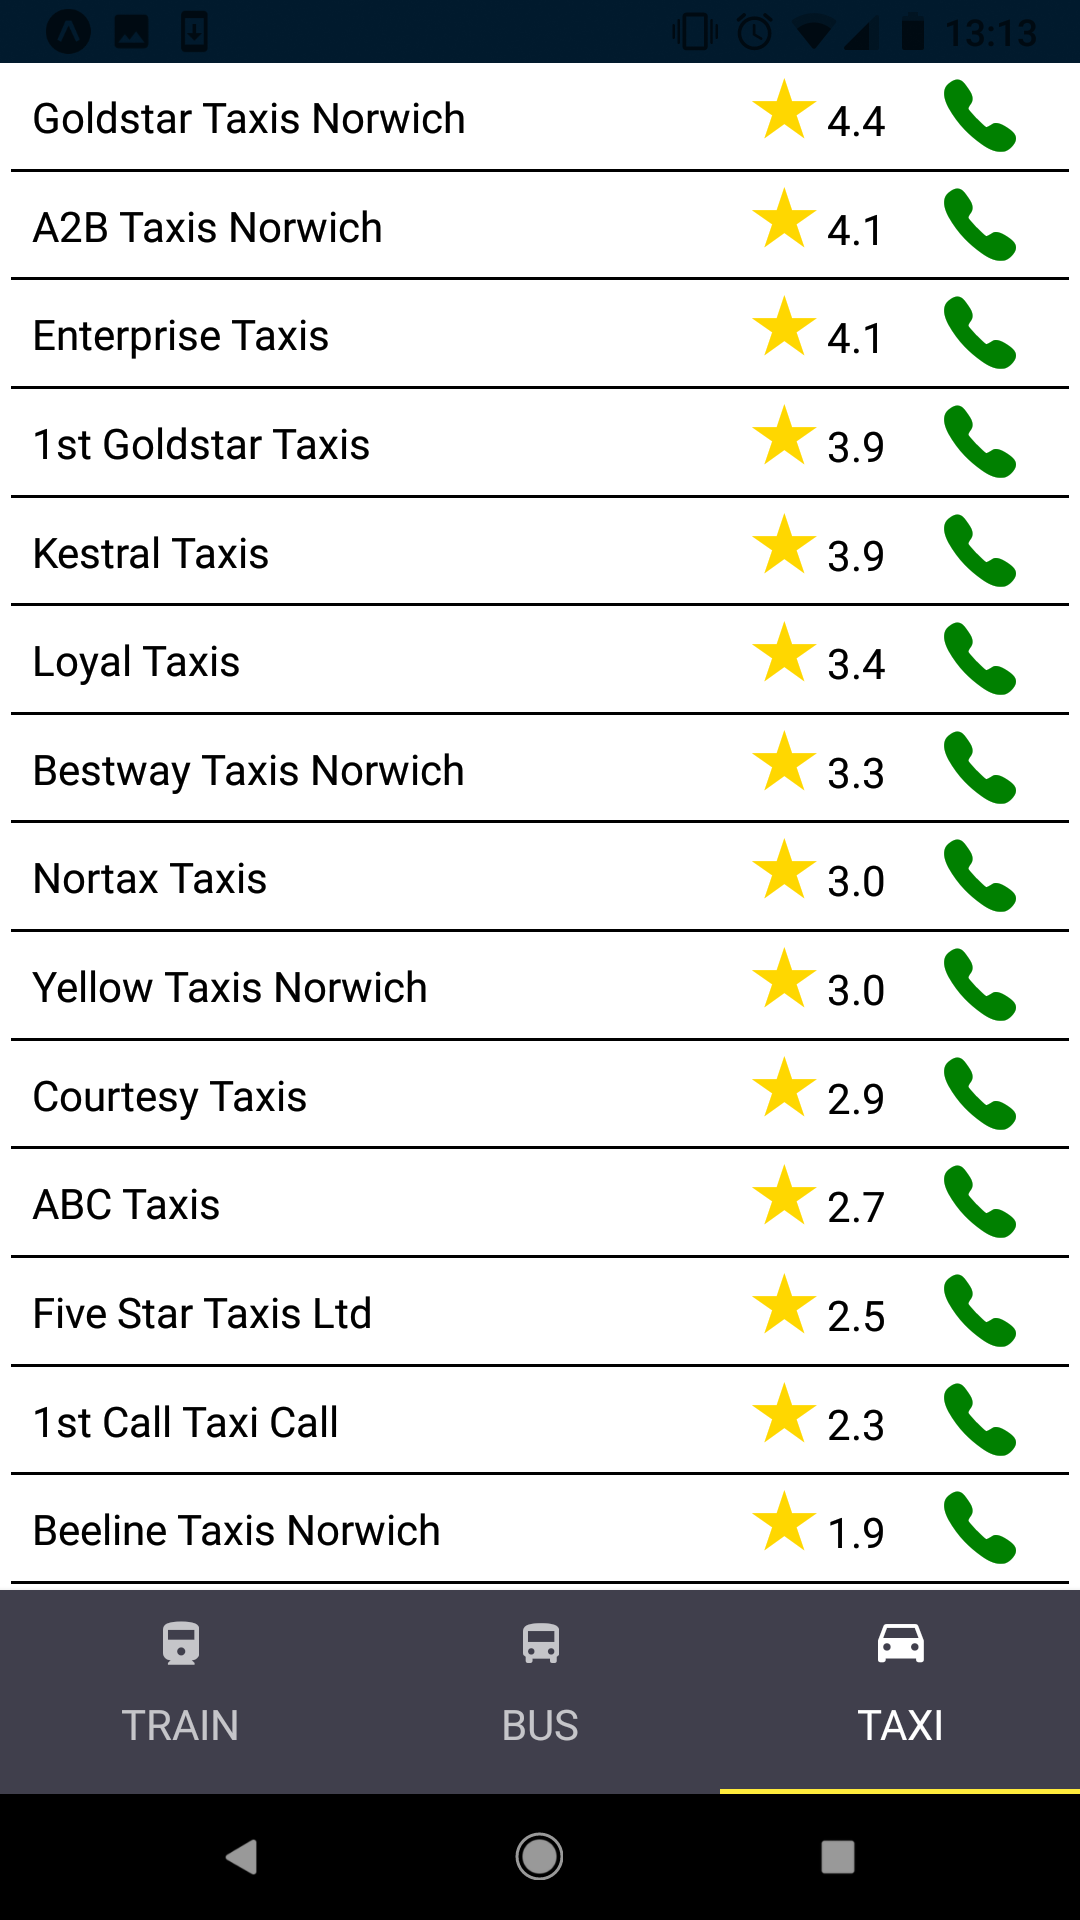
\includegraphics[height=10cm]{images/android-taxi.png}\\
			\caption{A screenshot taken from the android version of \nt \ showing the Taxi Screen, displaying the Taxi companies pulled from the Google Maps API then sorted by rating.}\label{fig:android-taxi}
		\end{figure}
		\begin{figure}[h]
			\centering
			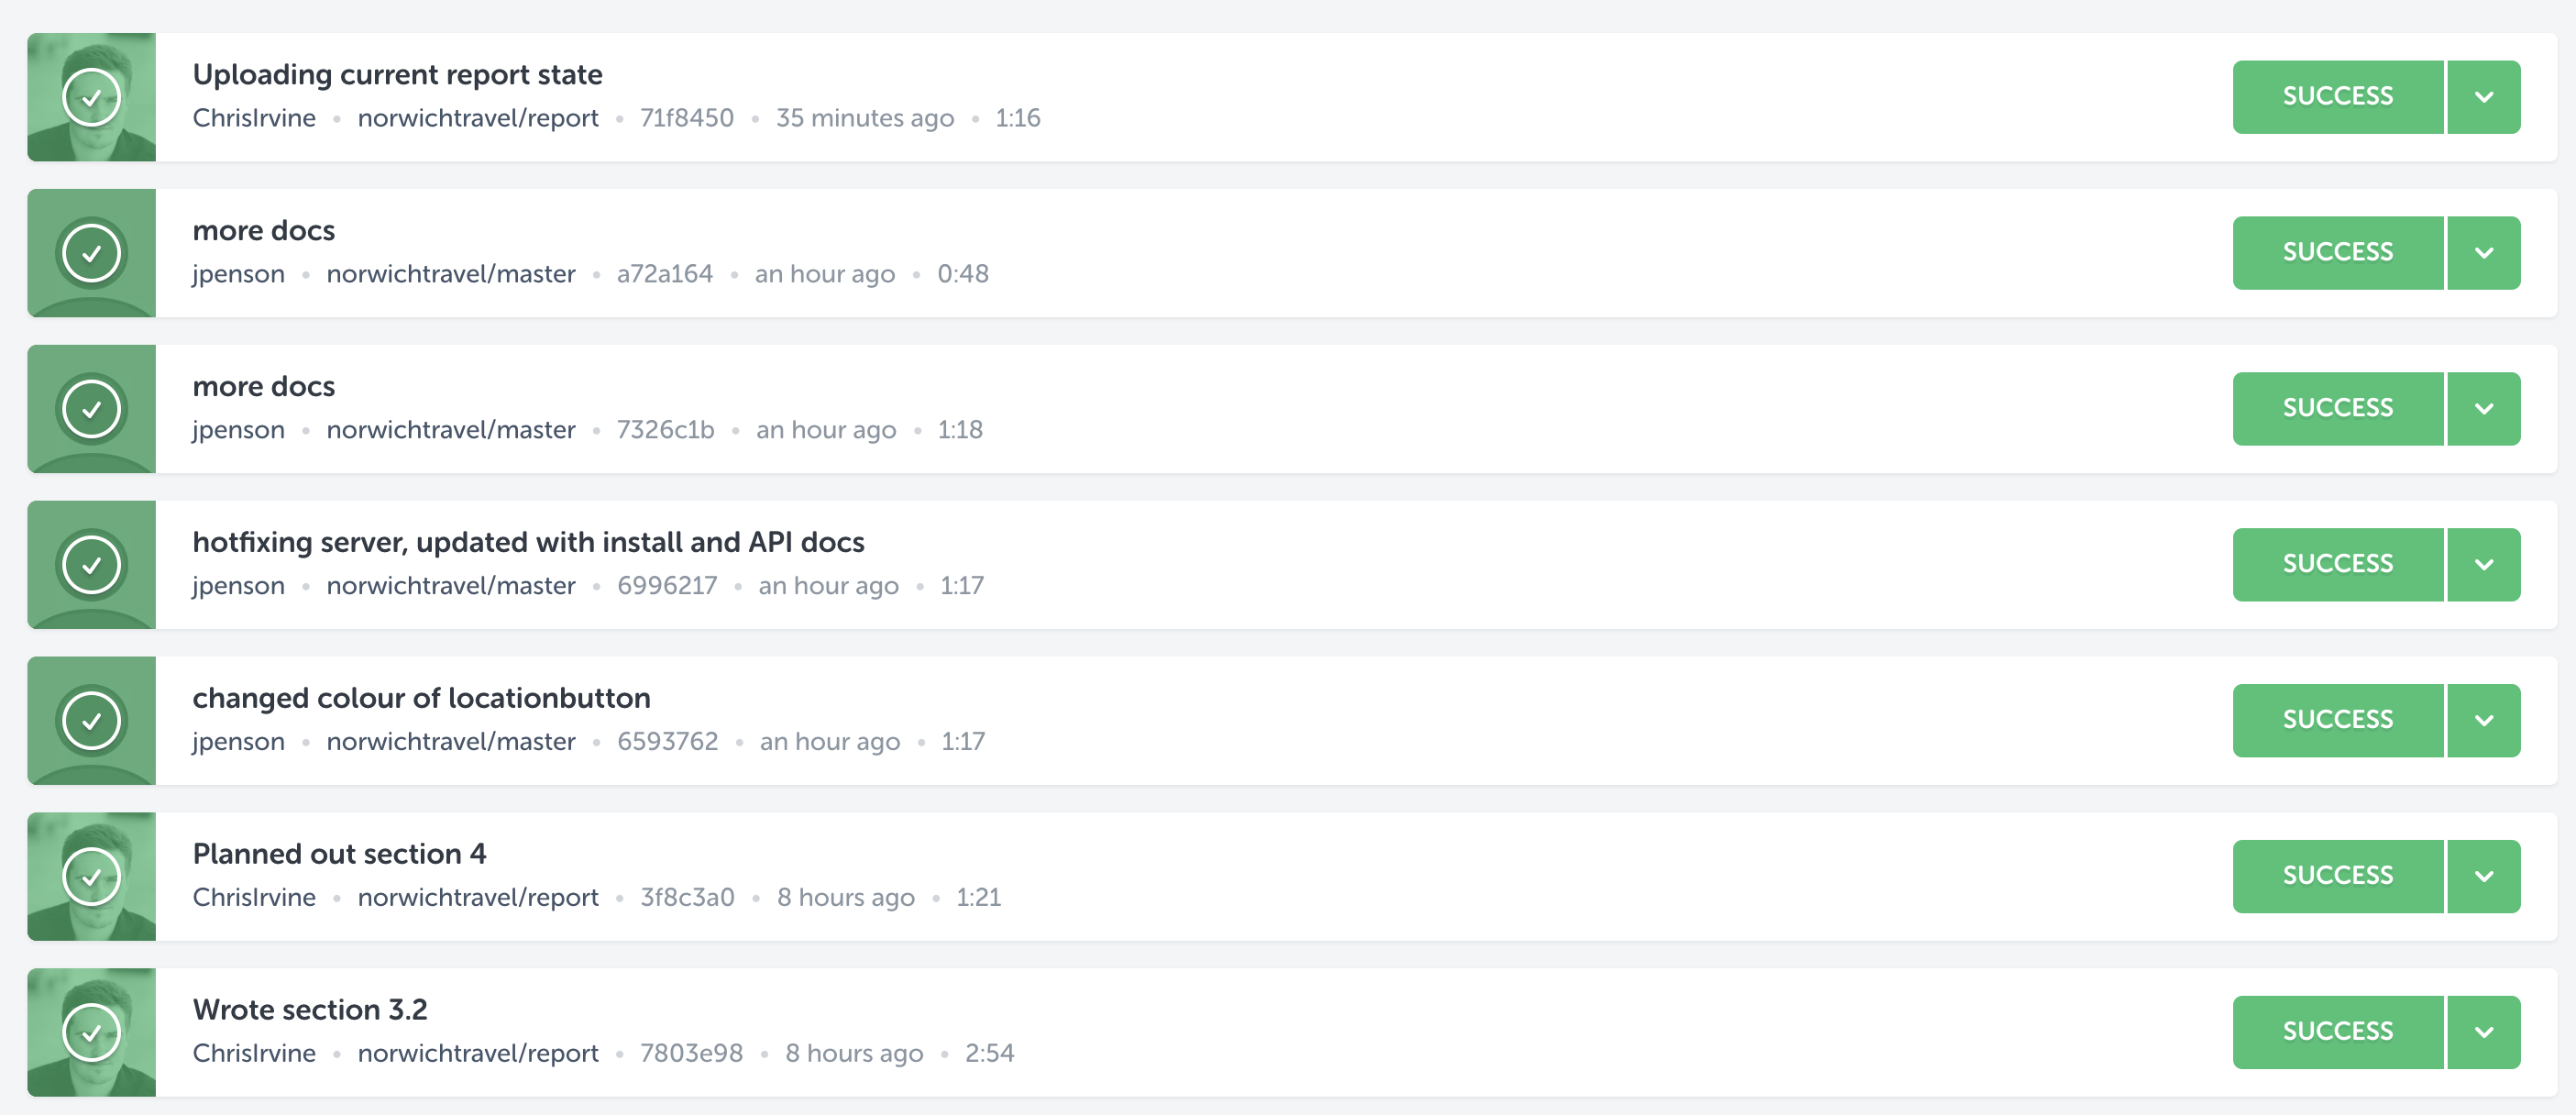
\includegraphics[height=6cm]{images/codeship.png}\\
			\caption{A screenshot taken Codeship showing the various tests and checks that \nt \ must pass through in order to be deployed.}\label{fig:codeship}
		\end{figure}
		\begin{figure}[h]
			\centering
			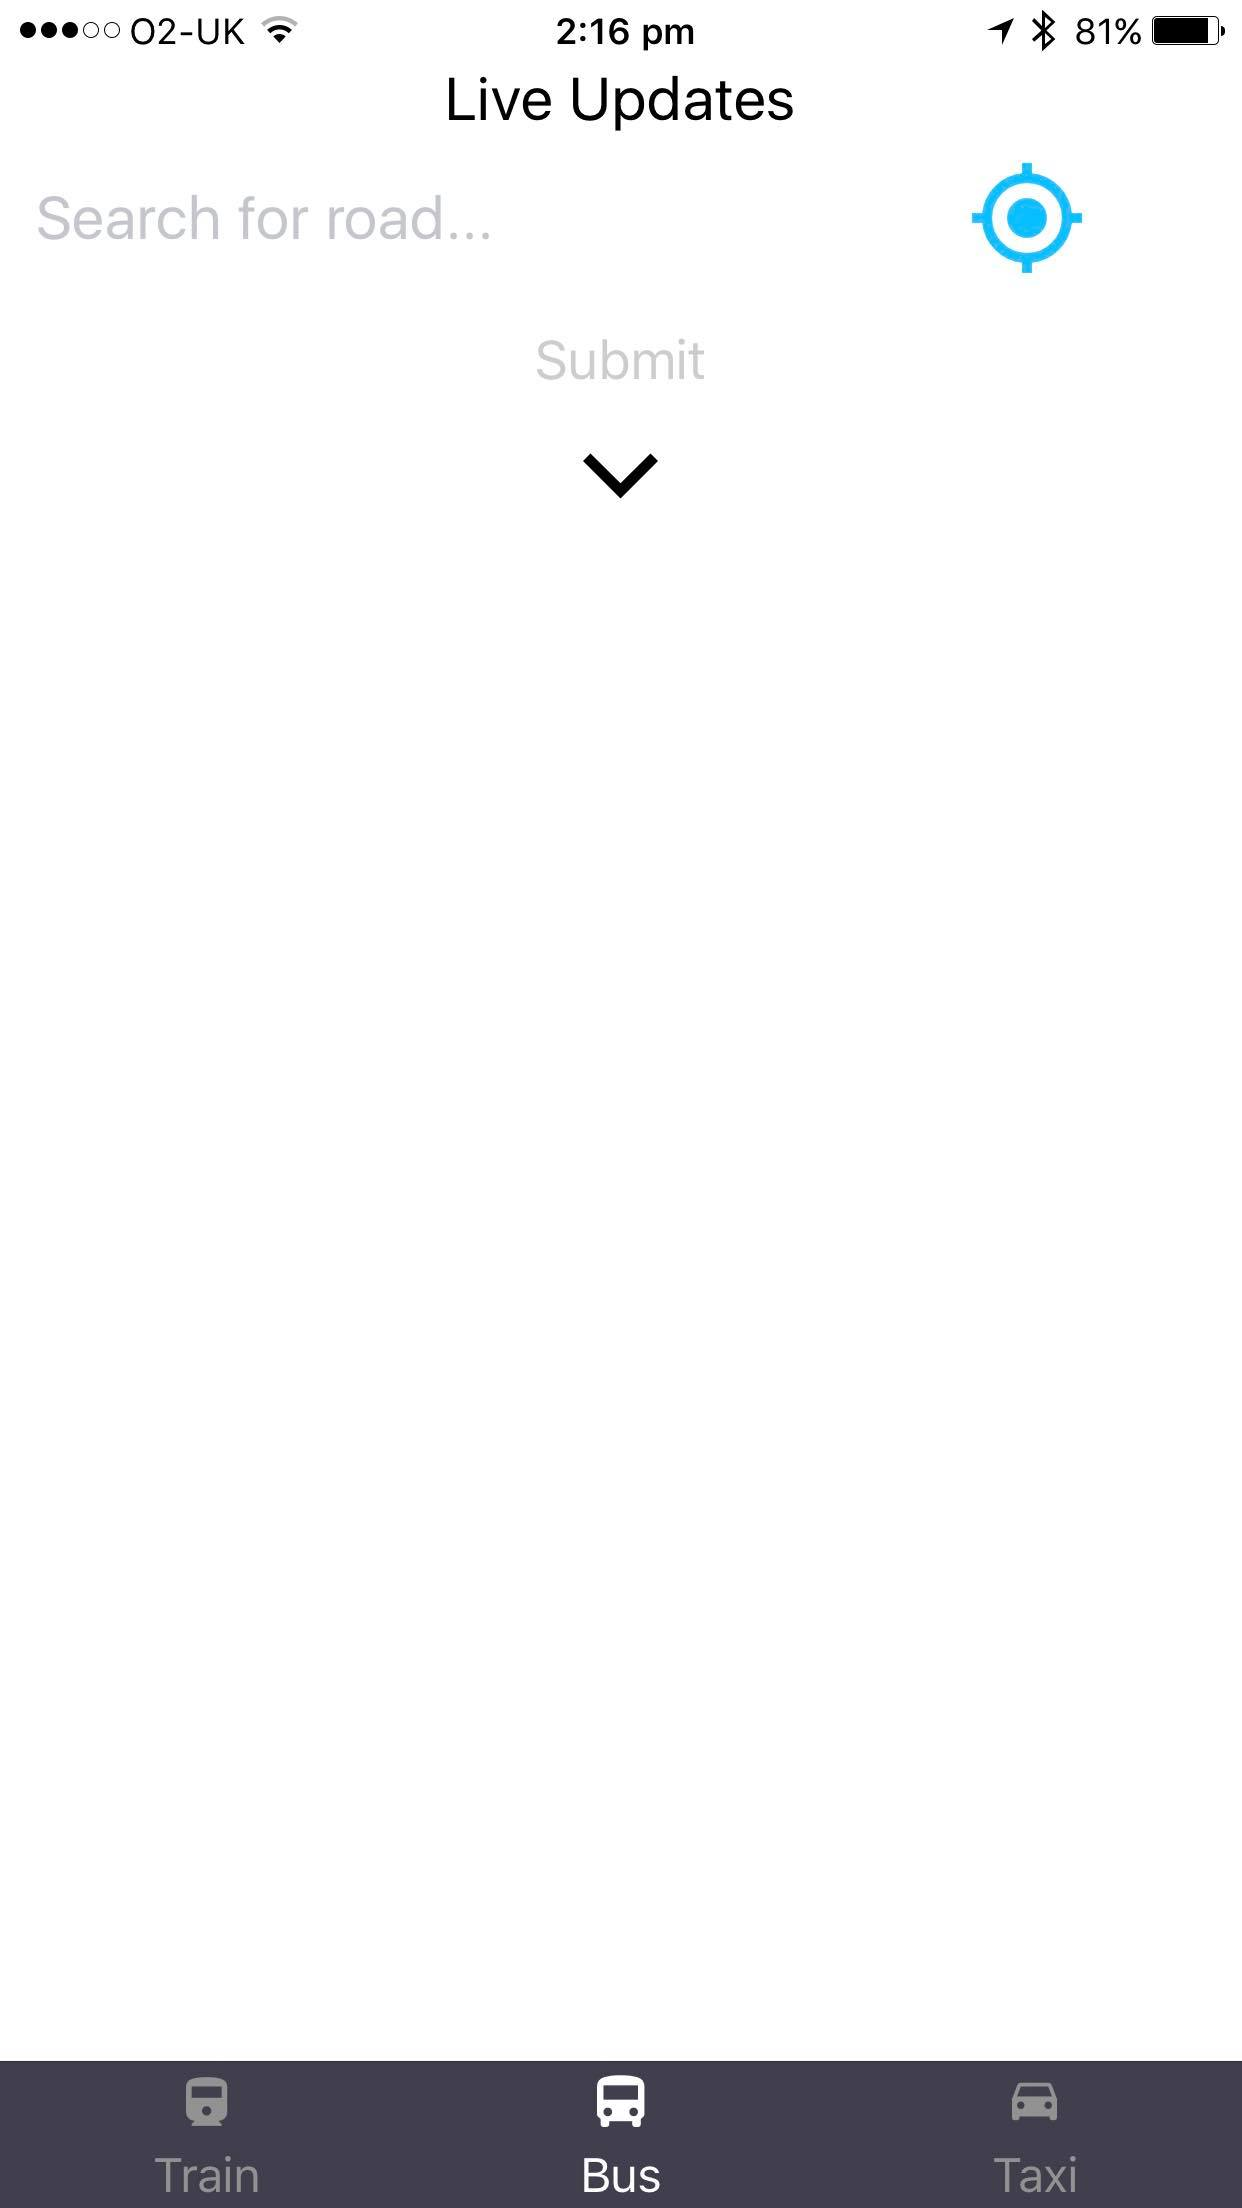
\includegraphics[height=10cm]{images/ios-landing.jpg}\\
			\caption{A screenshot taken from the iOS version of \nt \ showing the landing page that a User will first see when they open the app.}\label{fig:ios-landing}
		\end{figure}
		\begin{figure}[h]
			\centering
			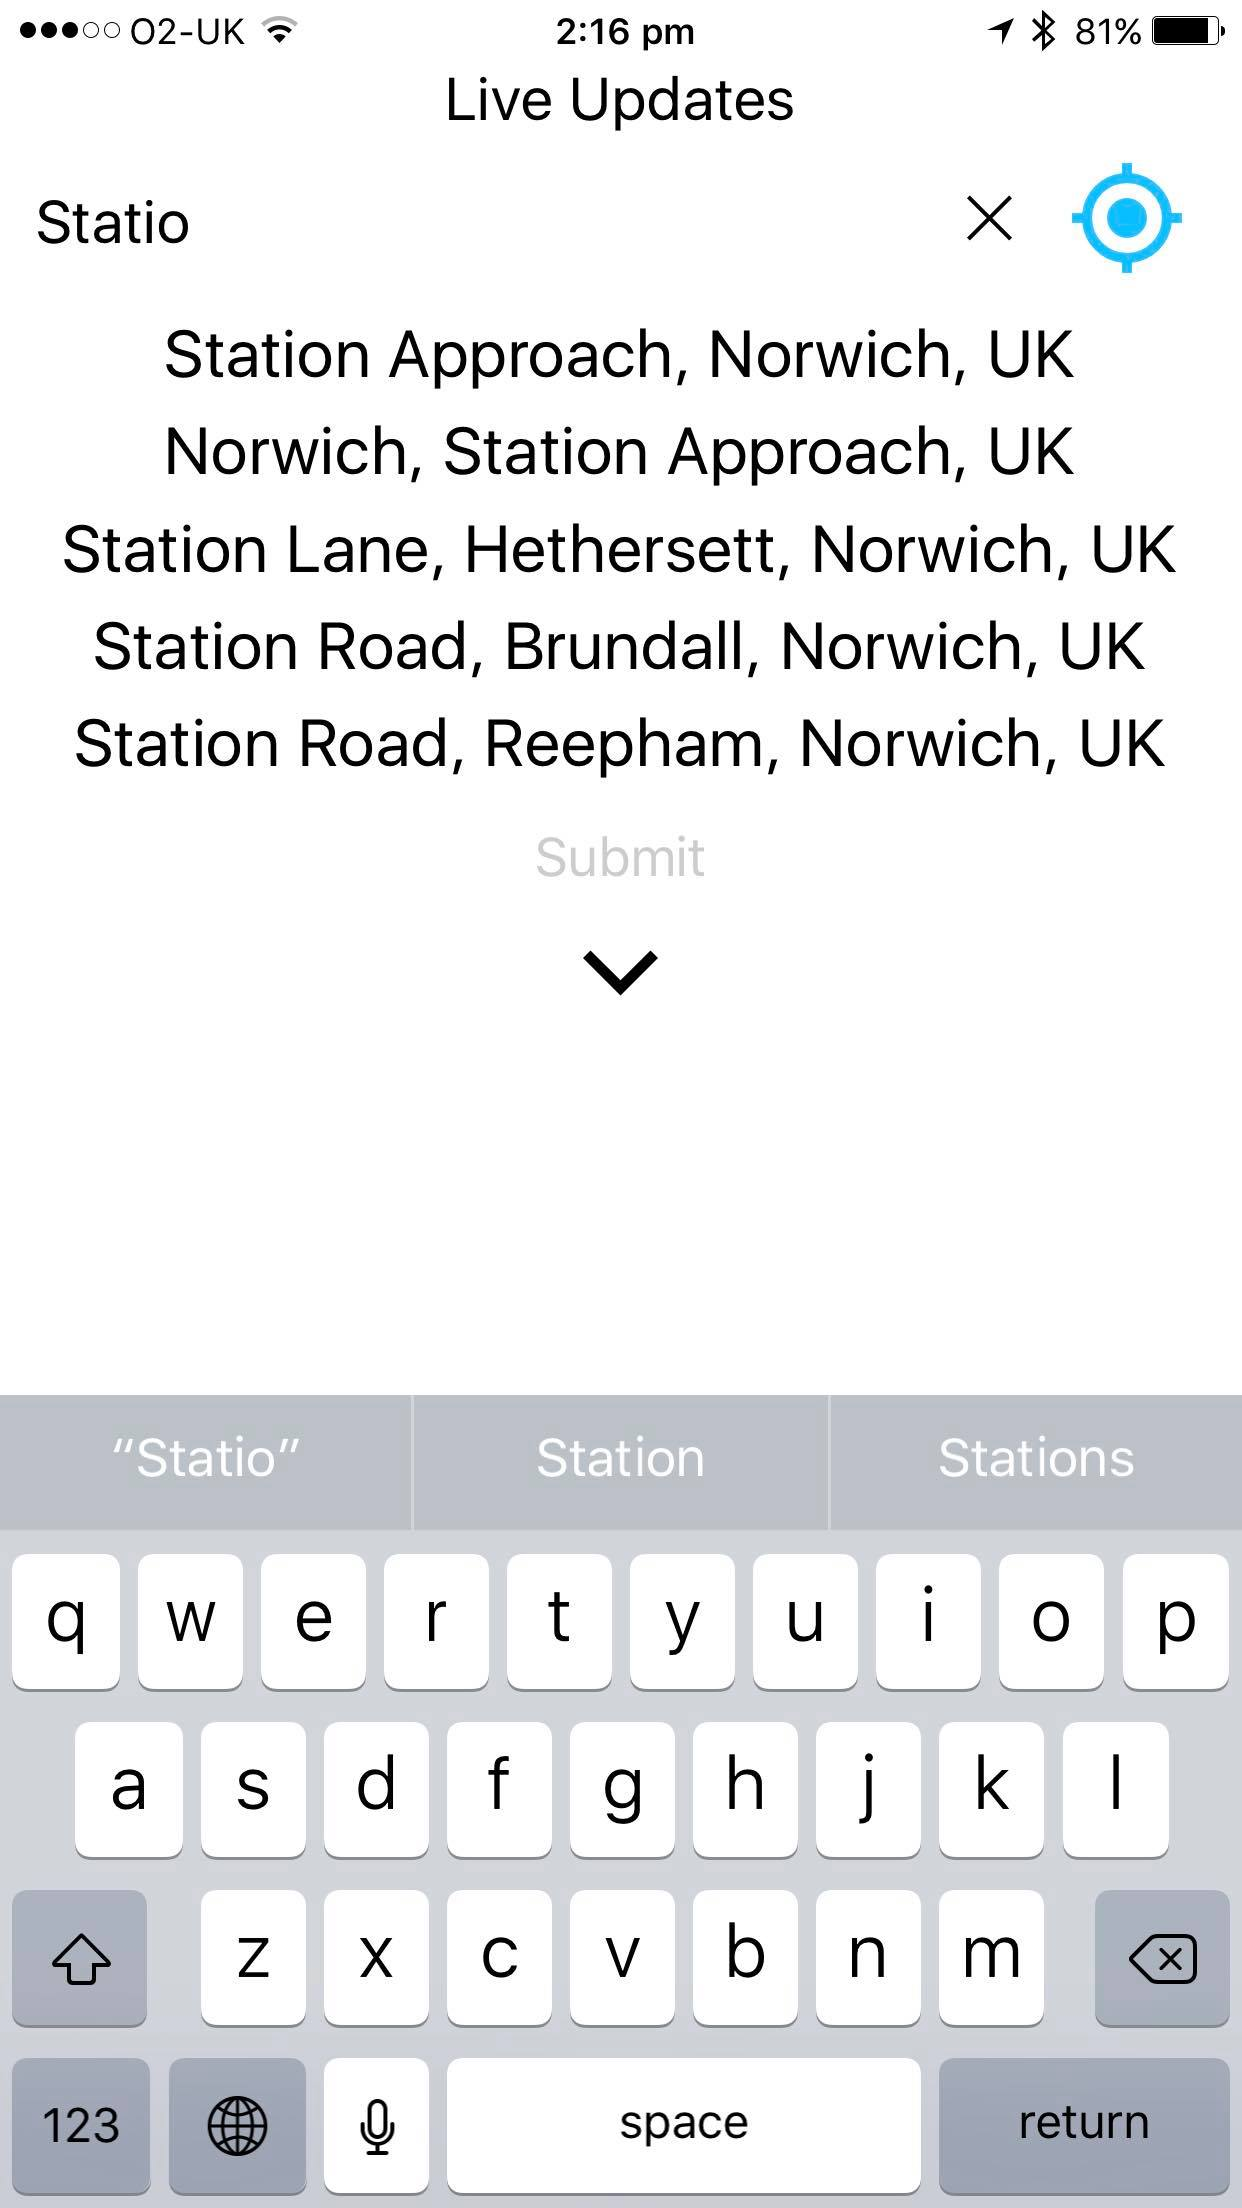
\includegraphics[height=10cm]{images/ios-bus-1.jpg}\\
			\caption{A screenshot taken from the iOS version of \nt \ showing the Bus Screen with the text field filled.}\label{fig:ios-bus-1}
		\end{figure}
		\begin{figure}[h]
			\centering
			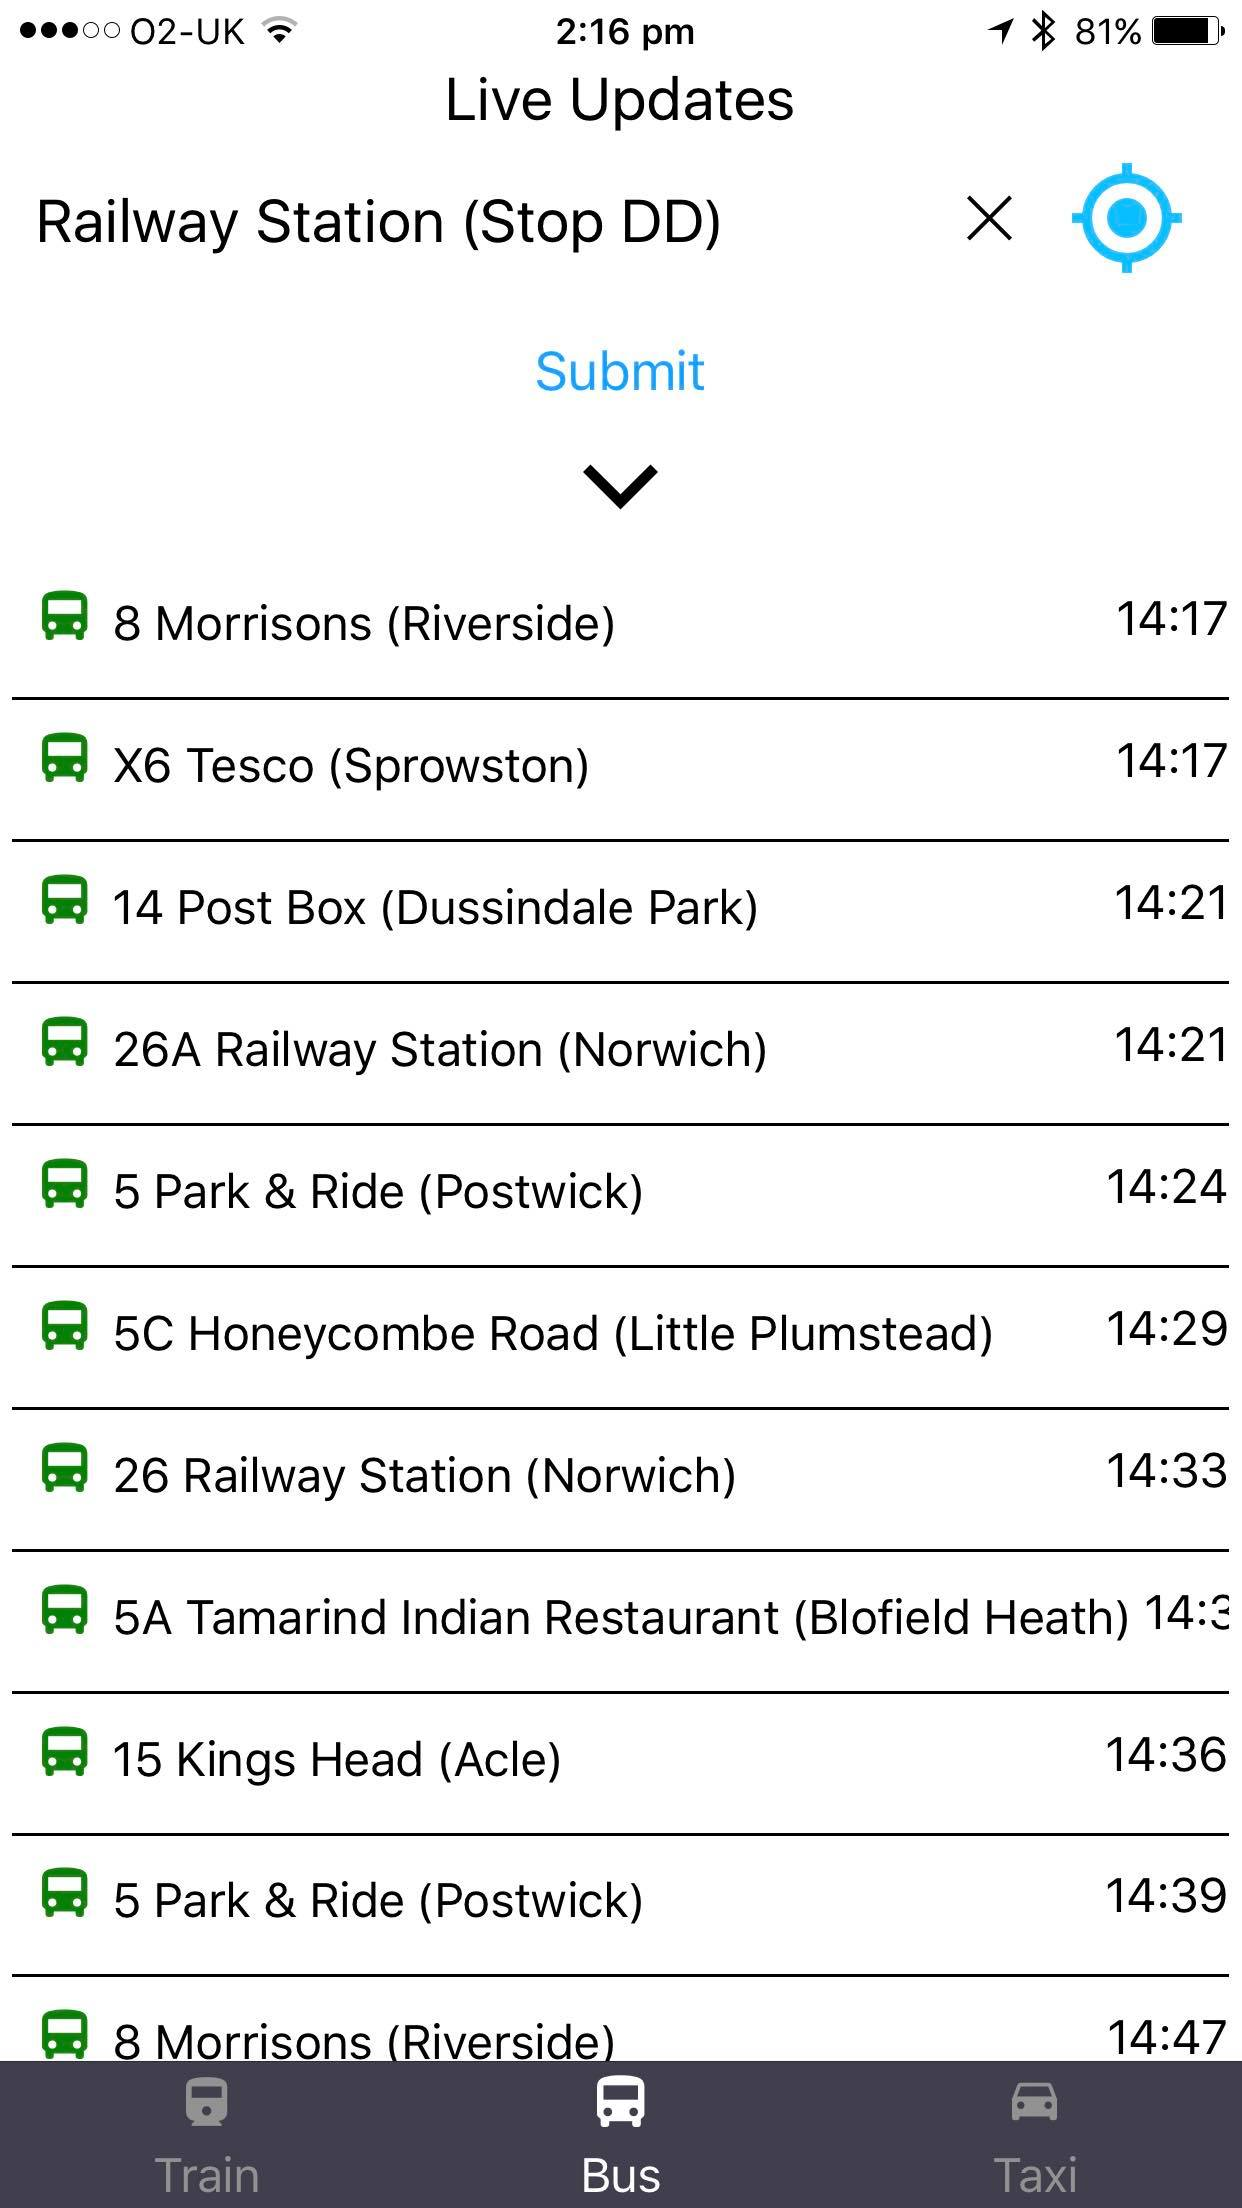
\includegraphics[height=10cm]{images/ios-bus-2.jpg}\\
			\caption{A screenshot taken from the iOS version of \nt \ showing the Bus Screen with the results generated.}\label{fig:ios-bus-2}
		\end{figure}
		\begin{figure}[h]
			\centering
			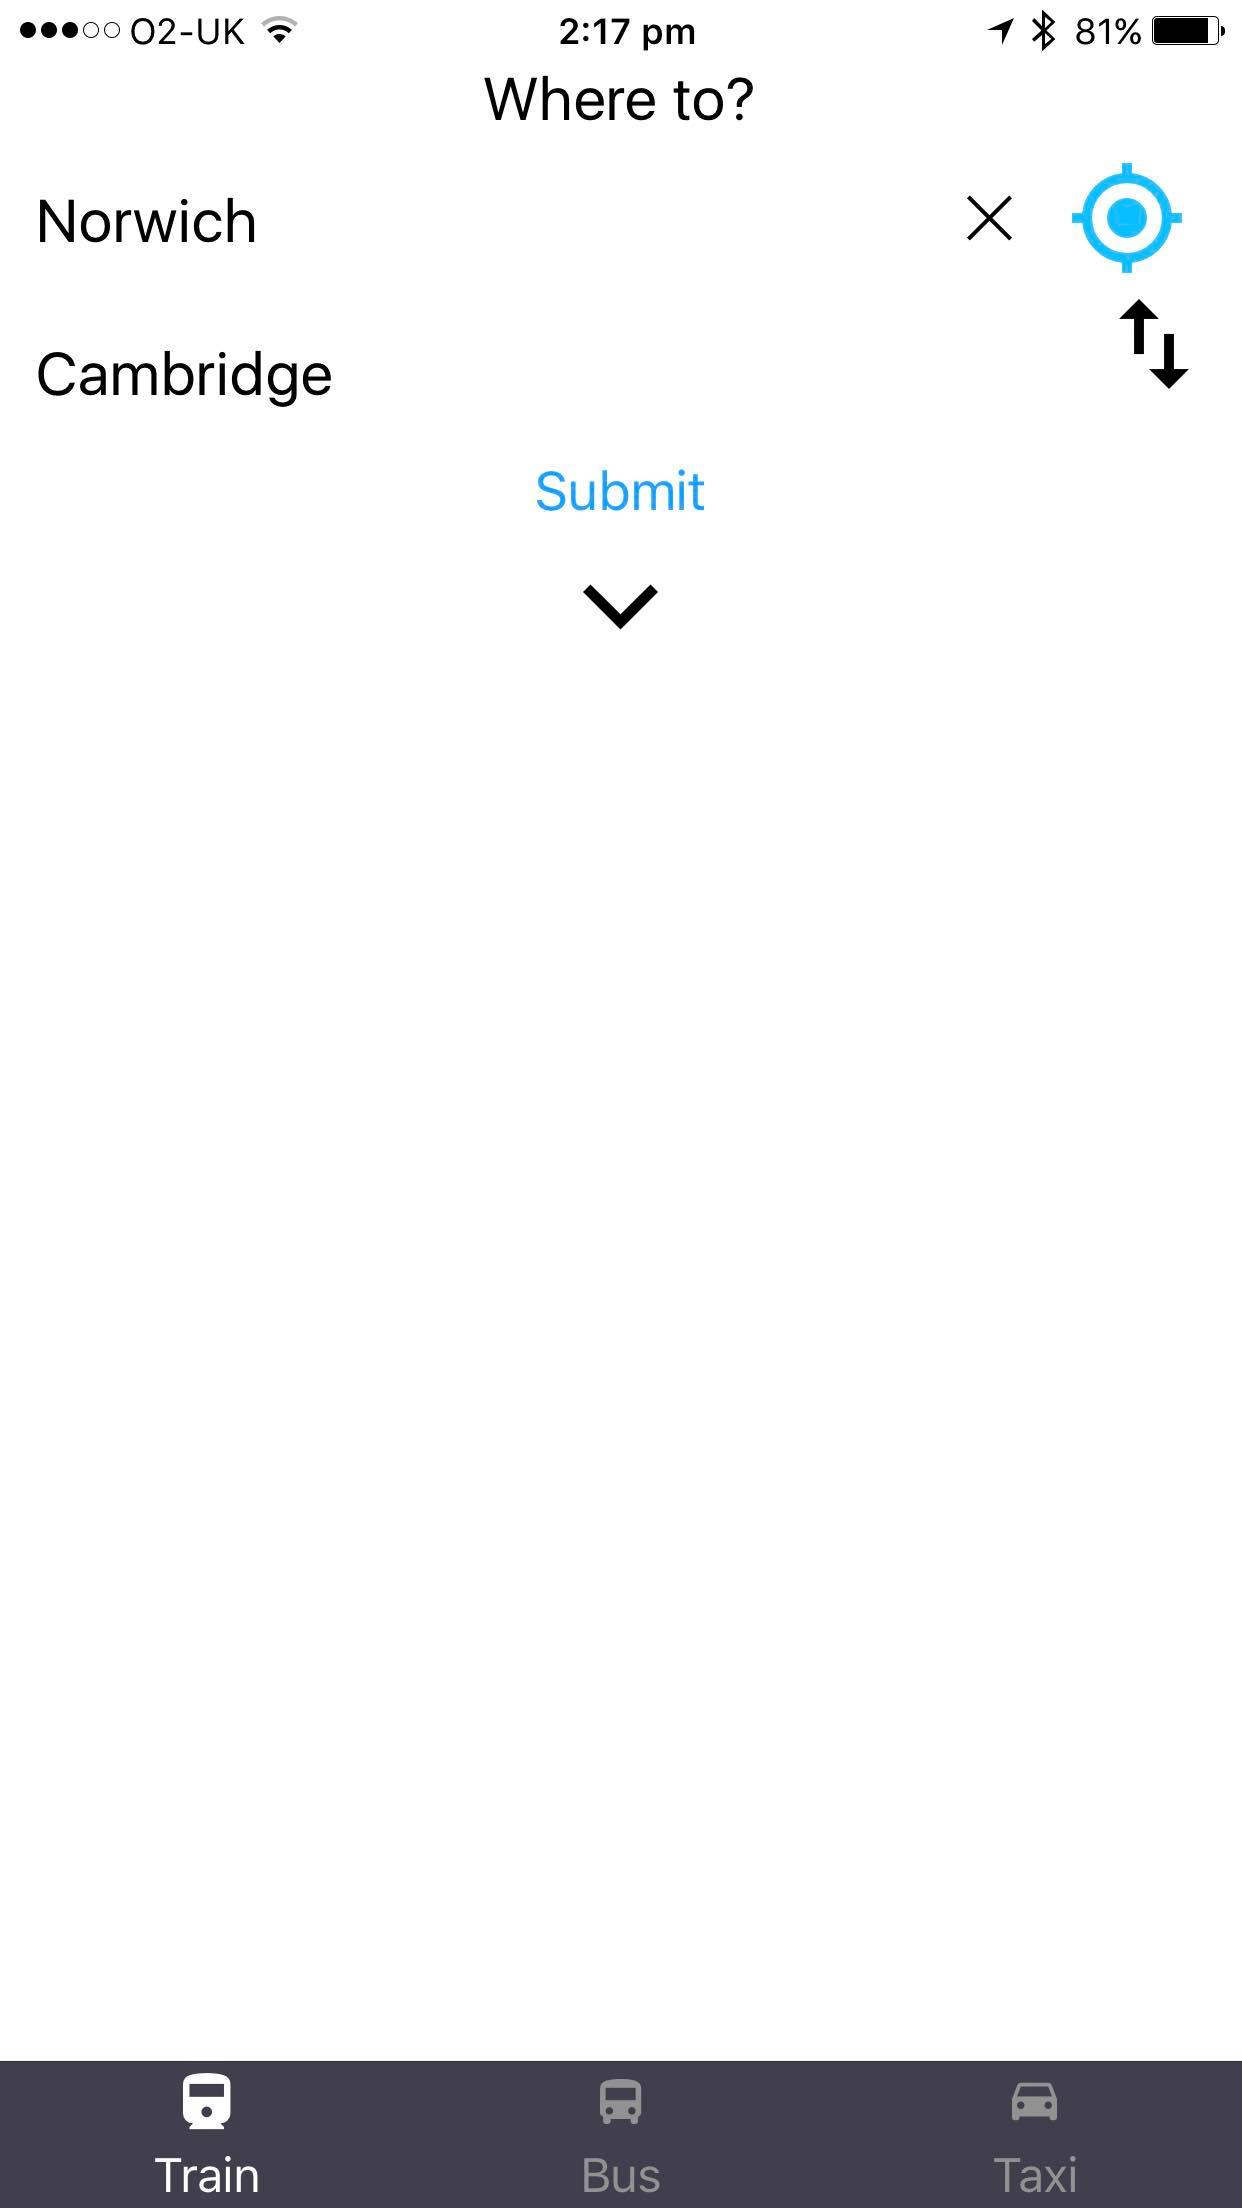
\includegraphics[height=10cm]{images/ios-train-1.jpg}\\
			\caption{A screenshot taken from the iOS version of \nt \ showing the Train Screen without anything entered. Norwich is the point of origin by default.}\label{fig:ios-train-1}
		\end{figure}
		\begin{figure}[h]
			\centering
			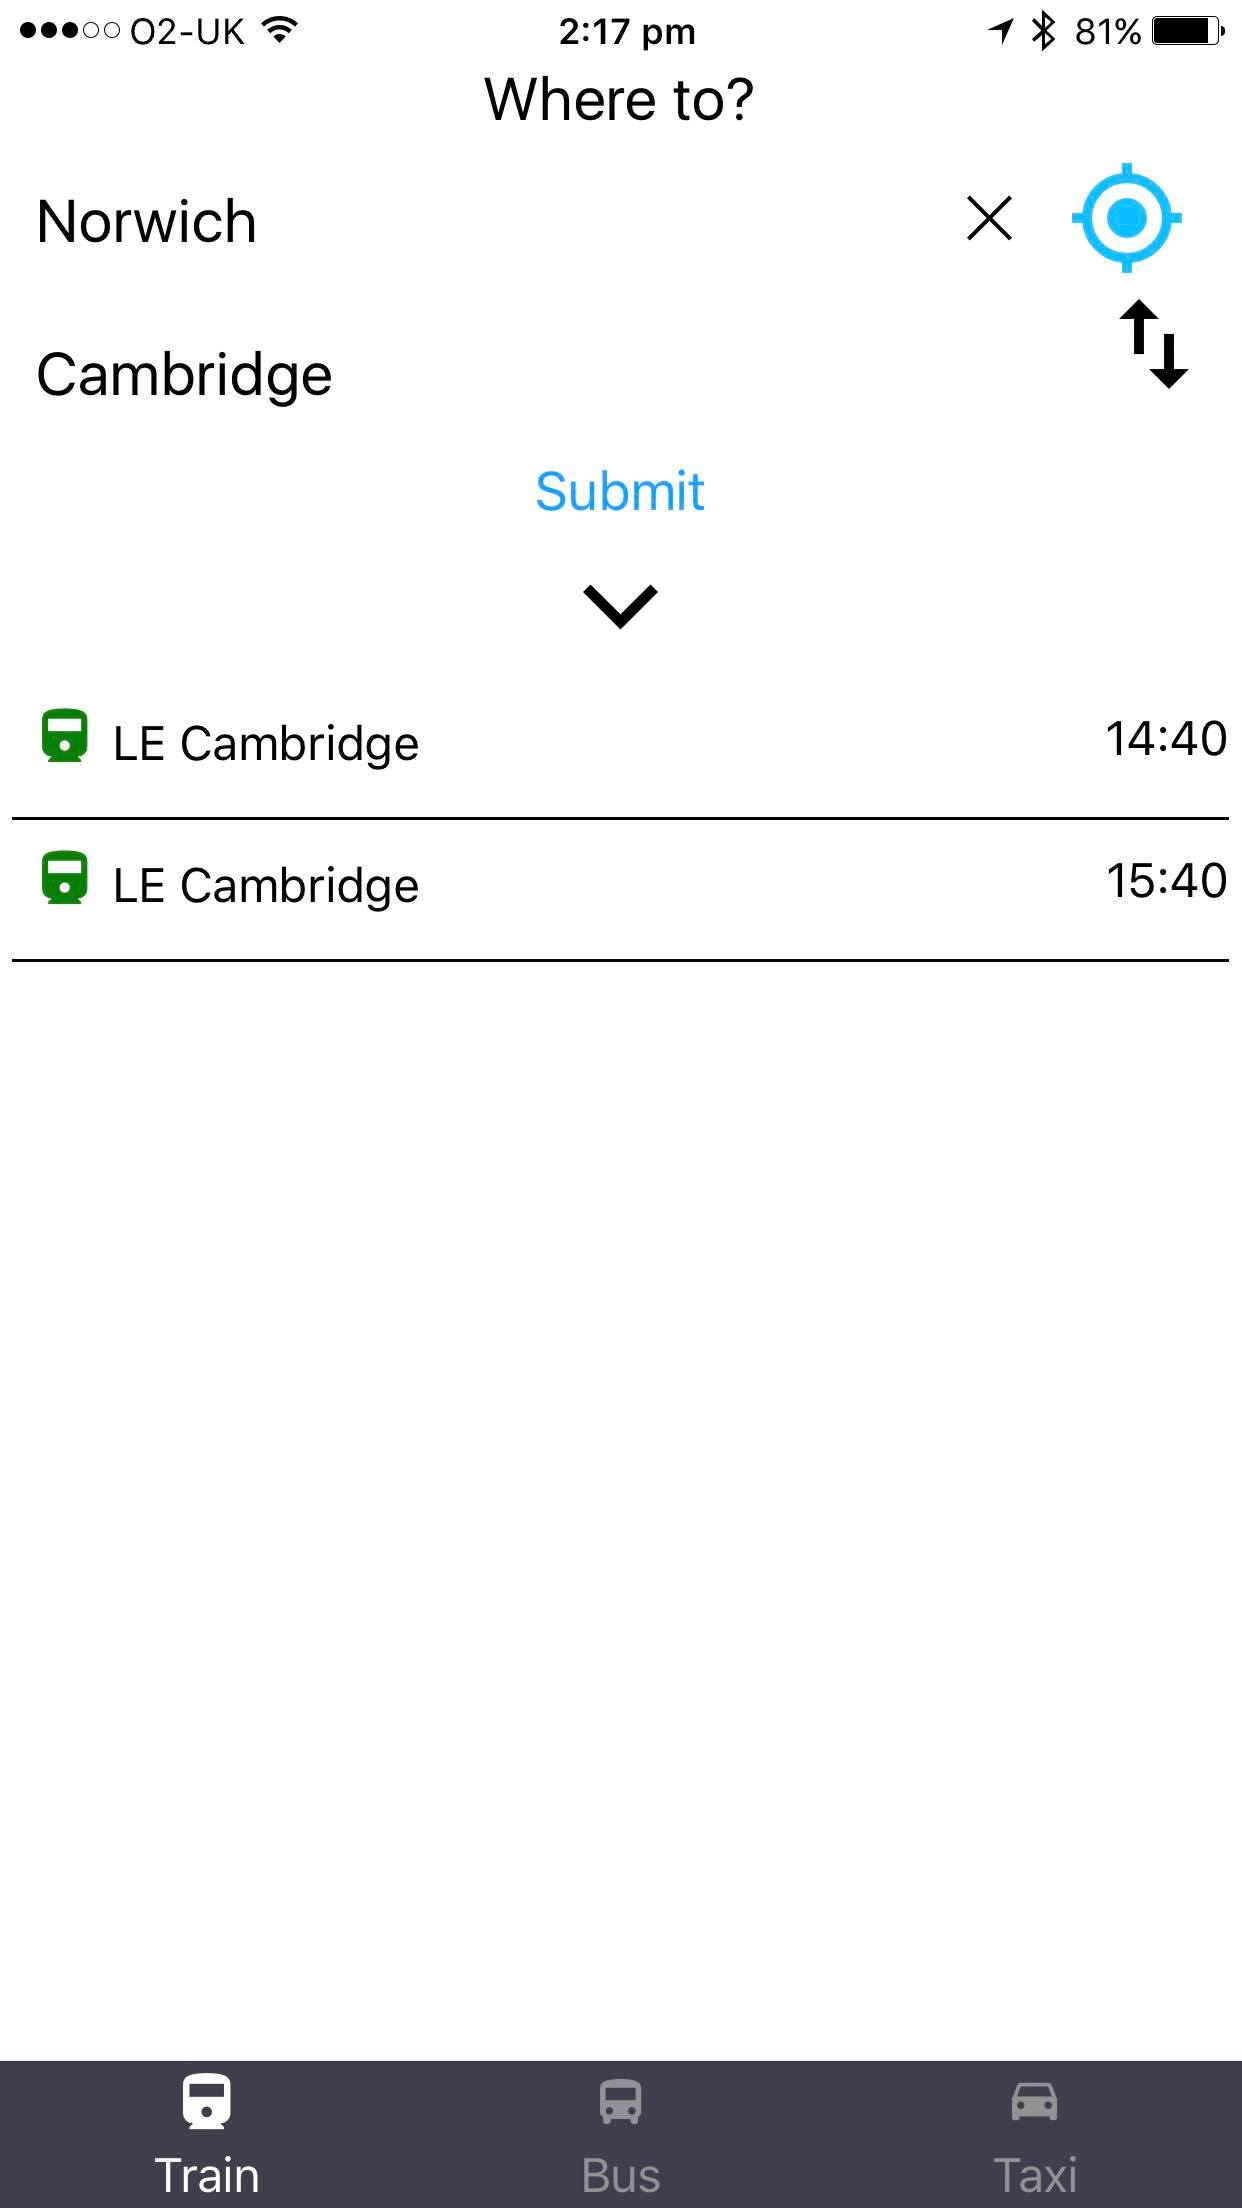
\includegraphics[height=10cm]{images/ios-train-2.jpg}\\
			\caption{A screenshot taken from the iOS version of \nt \ showing the Train Screen displaying the next rains leaving the station.}\label{fig:ios-train-2}
		\end{figure}
		\begin{figure}
			\centering
			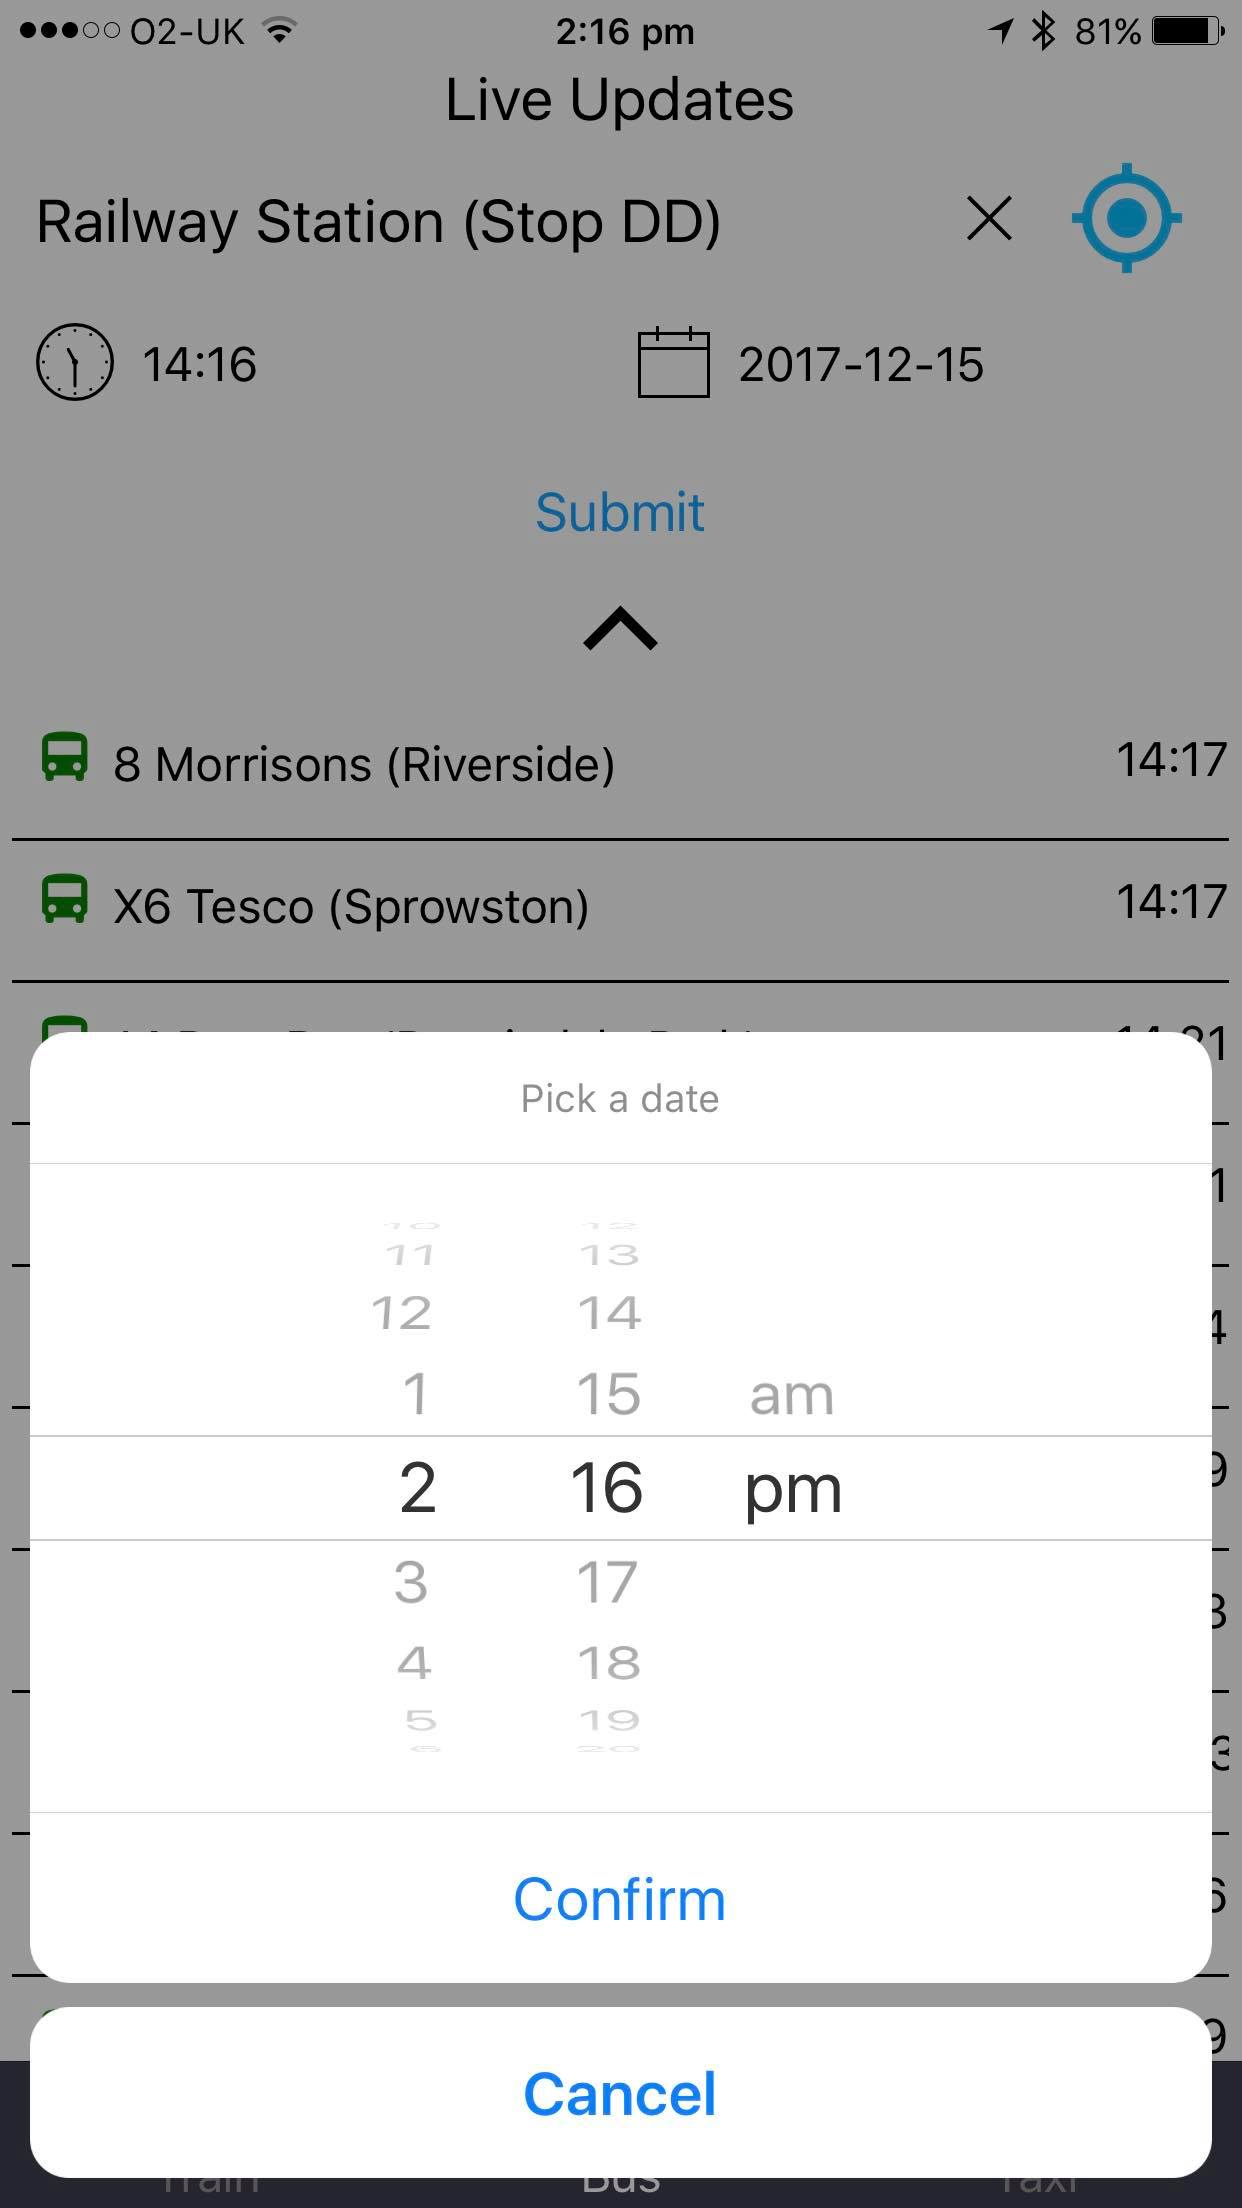
\includegraphics[height=10cm]{images/ios-time.jpg}\\
			\caption{A screenshot taken from the iOS version of \nt \ showing the iOS native time selector.}\label{fig:ios-time}
		\end{figure}
		\begin{figure}
			\centering
			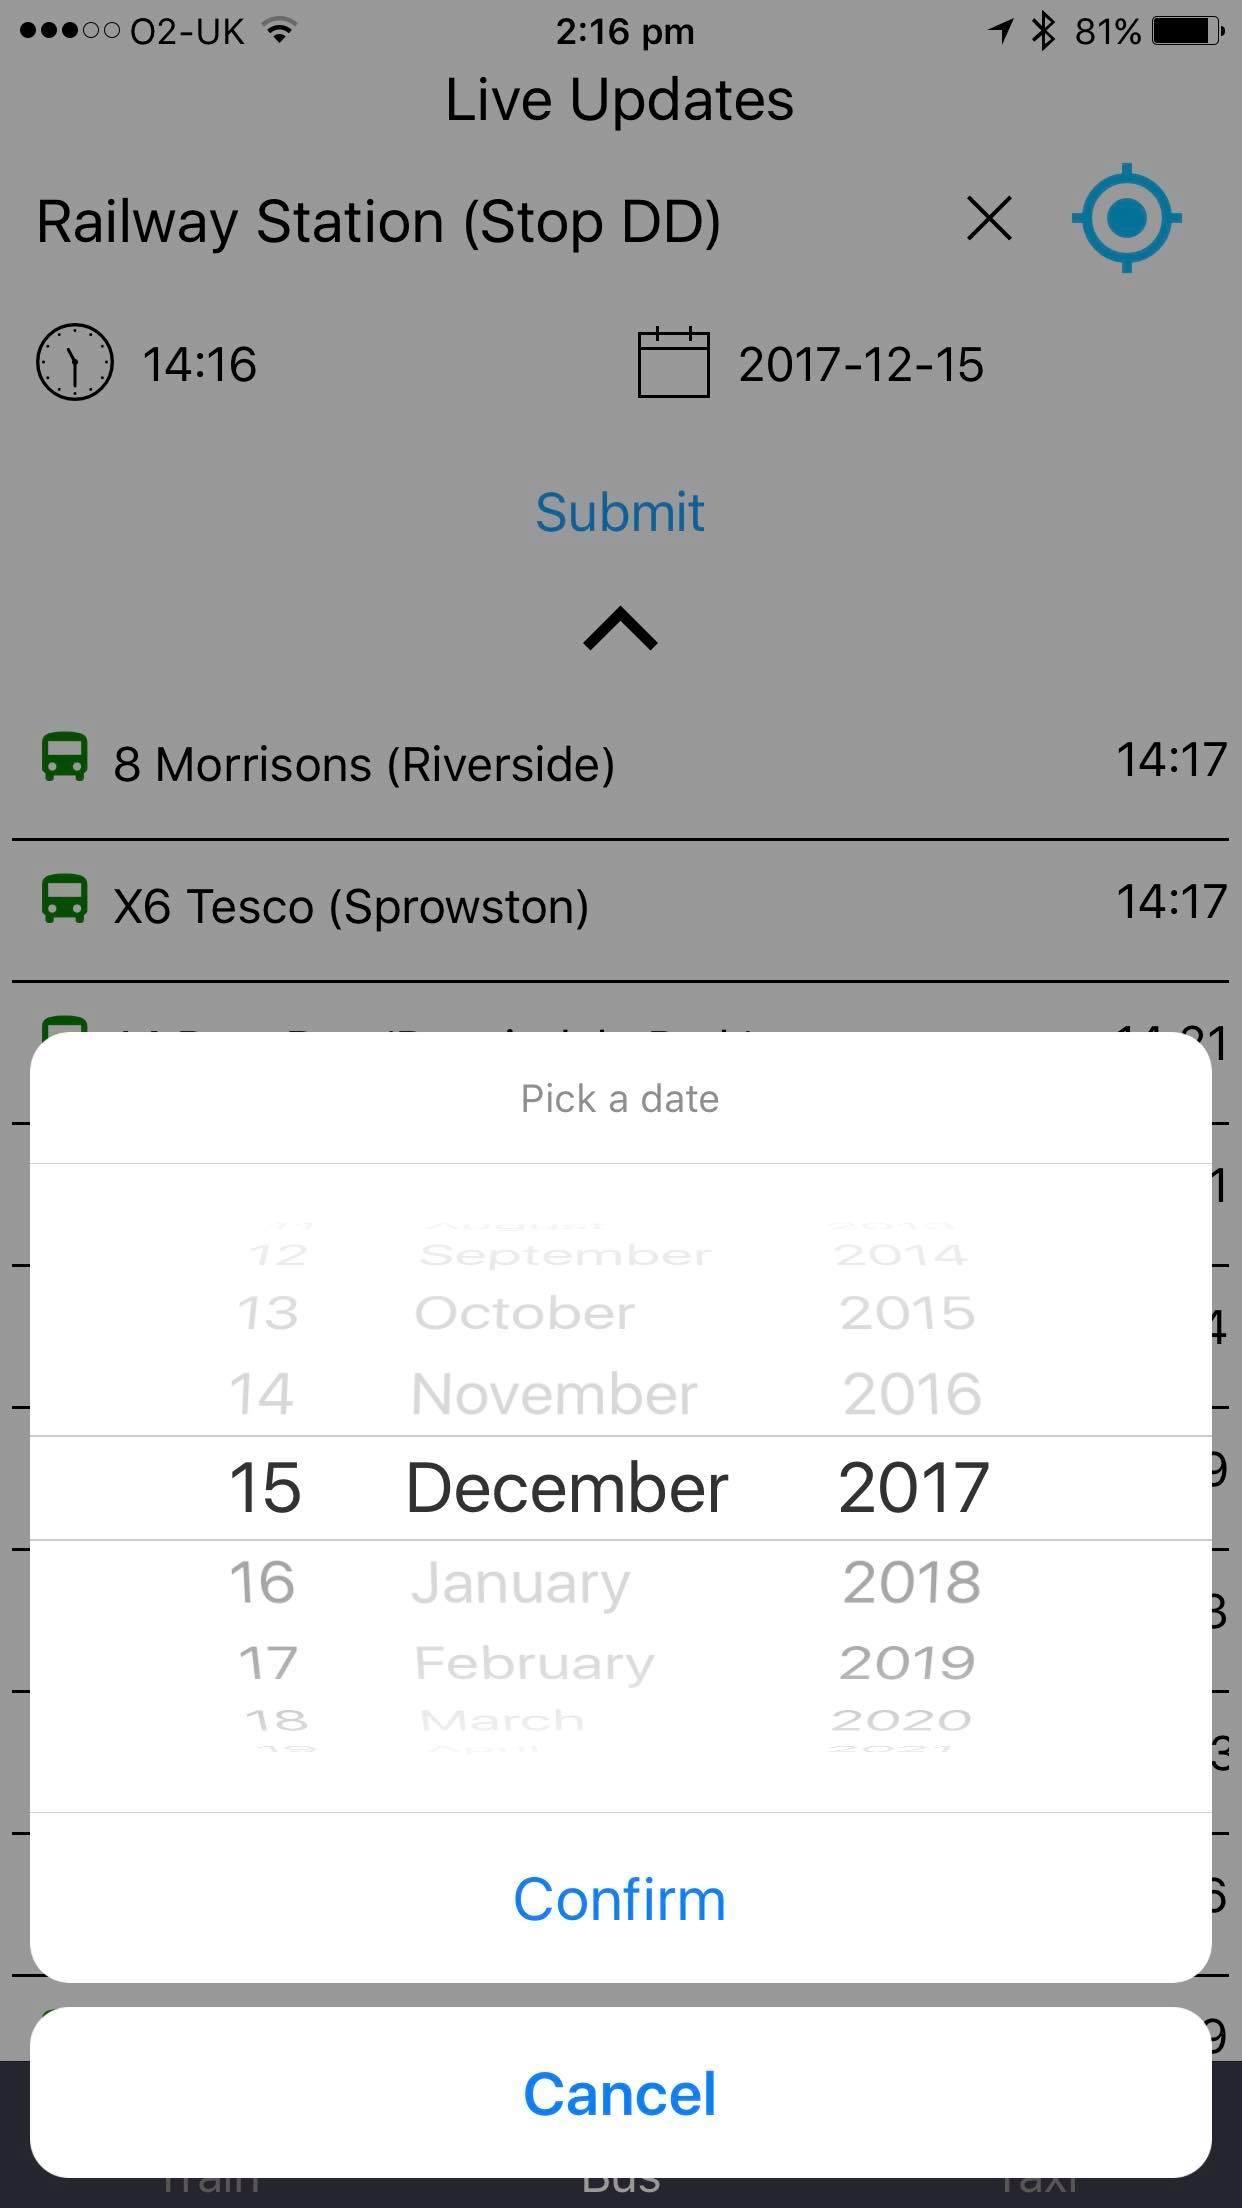
\includegraphics[height=10cm]{images/ios-date.jpg}\\
			\caption{A screenshot taken from the iOS version of \nt \ showing the iOS native date selector.}\label{fig:ios-date}
		\end{figure}
		\begin{figure}[h]
			\centering
			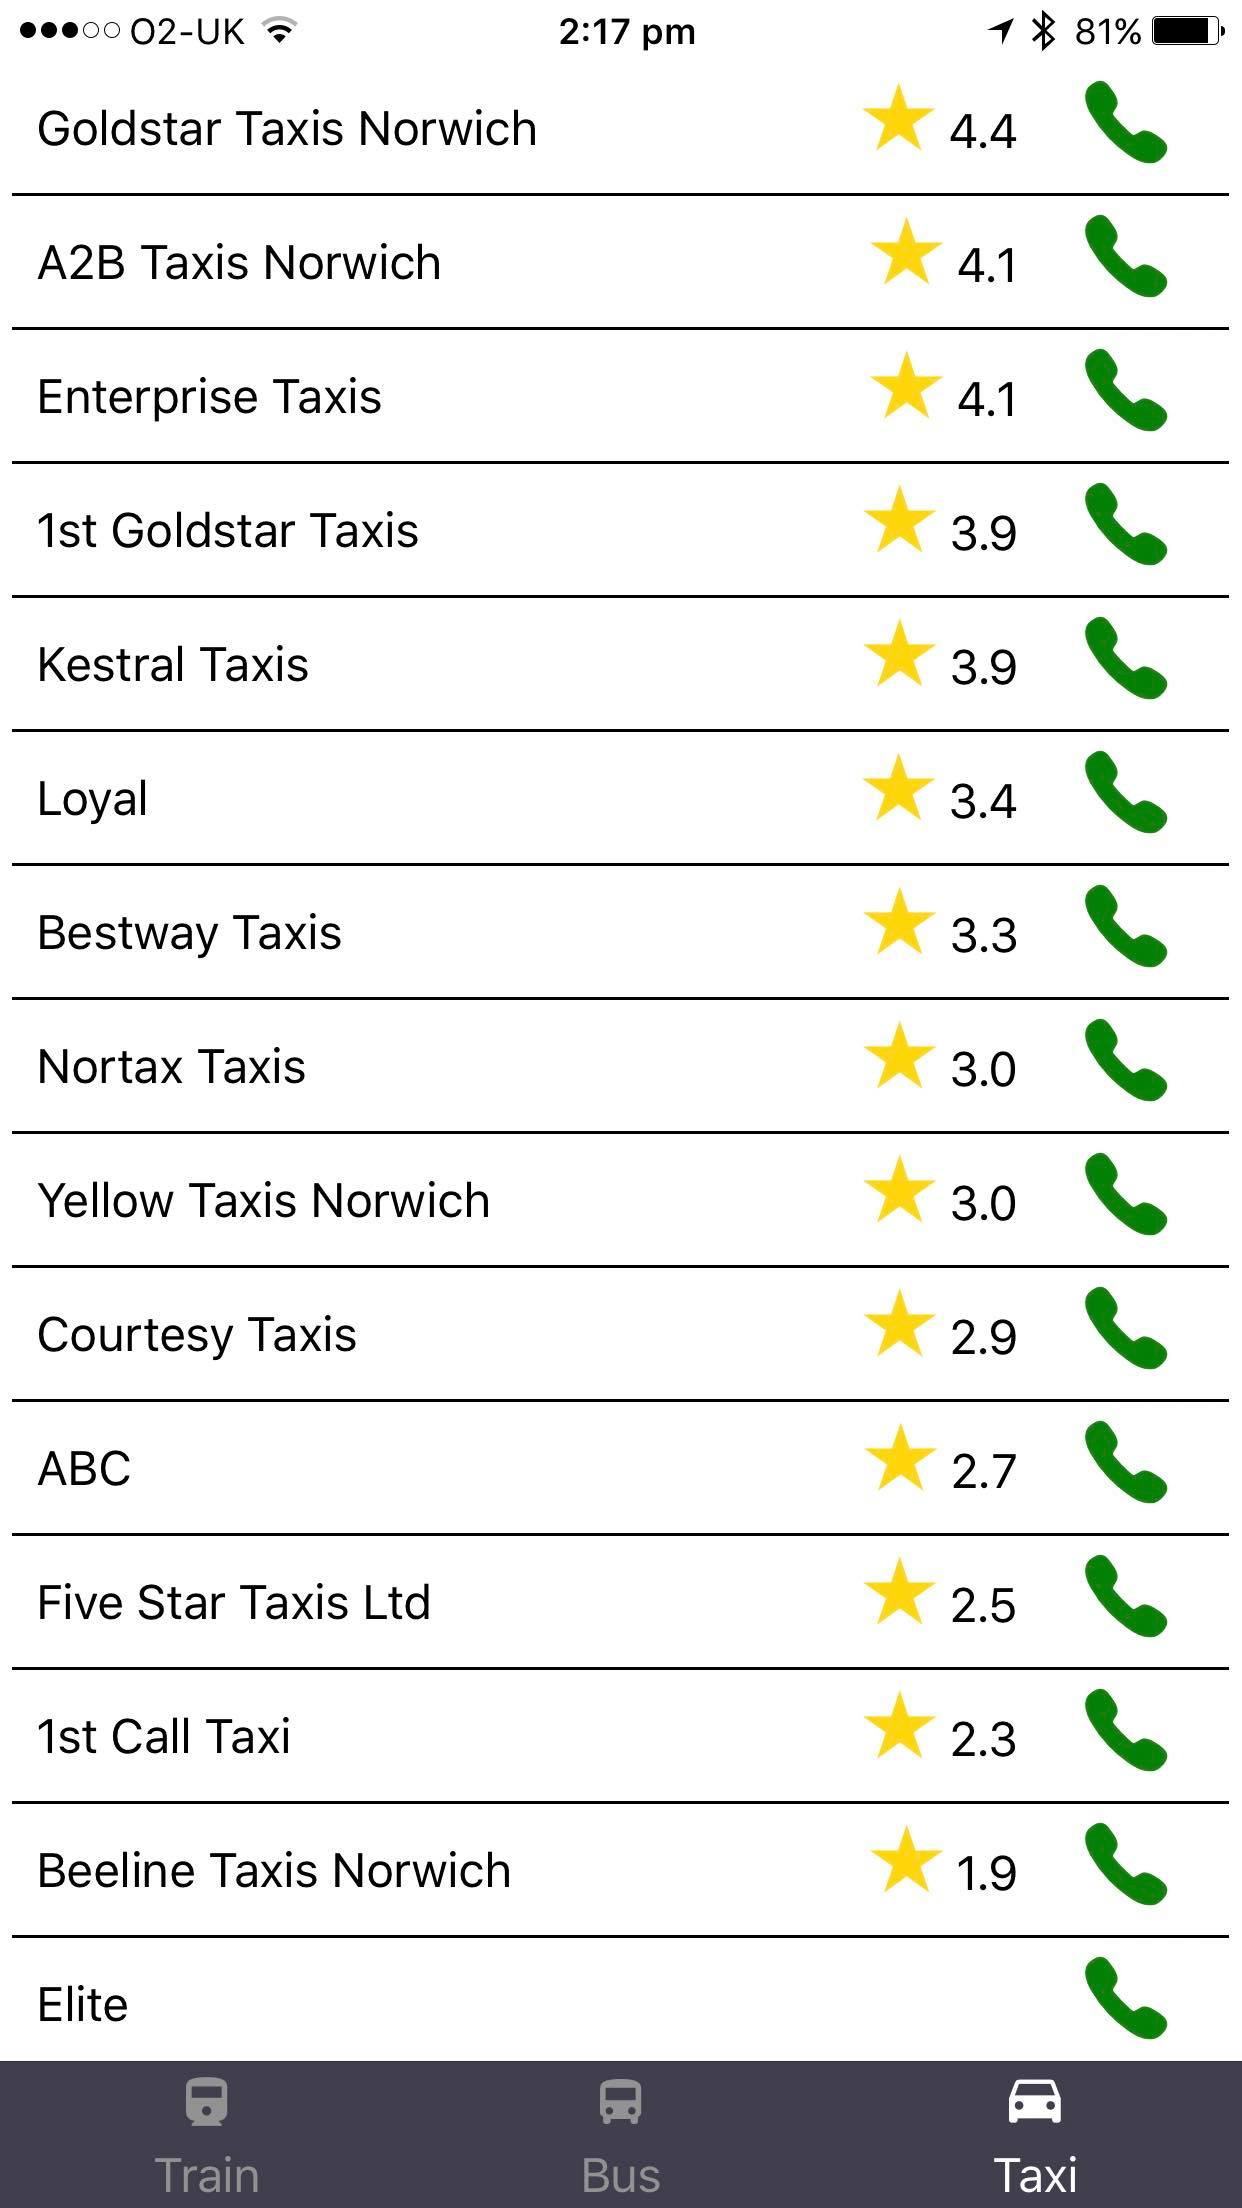
\includegraphics[height=10cm]{images/ios-taxi.jpg}\\
			\caption{A screenshot taken from the iOS version of \nt \ showing the Taxi Screen, displaying the Taxi companies pulled from the Google Maps API then sorted by rating.}\label{fig:ios-taxi}
		\end{figure}
	\clearpage
	\section{UML Diagrams}
		\begin{figure}[h]
			\centering
			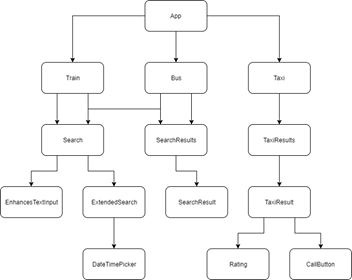
\includegraphics[height=10cm]{images/object-orientated.png}\\
			\caption{UML Diagram showing the organisation of \nt.}\label{fig:oo}
		\end{figure}
\end{document}

% EOF Document